\documentclass[a4paper]{article}
\usepackage{amsmath}
\usepackage{ifluatex}
\ifluatex
 \usepackage{fontspec}
  %\setmainfont[Ligatures=TeX]{xits}
  %\setmathfont[math-style=ISO]{xits-math}
 \setmainfont[Ligatures=TeX]{Latin Modern Roman}
 \fontspec[SmallCapsFeatures={Letters=SmallCaps}]{Latin Modern Roman}
 \usepackage{unicode-math}
 \setmathfont[math-style=ISO]{latinmodernmath-regular.otf}
 %\setmathfont[math-style=ISO]{xits-math.otf}
\else
 \usepackage[utf8]{inputenc}
\fi

%\def\pgfsysdriver{pgfsys-tex4ht.def} % force htlatex to generate svg from tikz figures
\usepackage{microtype}
\usepackage{html}
\usepackage{graphicx}
\usepackage{tikz}
\usepackage{hyperref}
\usepackage[top=0.1\paperheight, bottom=0.1\paperheight, left=0.1\paperwidth, right=0.1\paperwidth]{geometry}
\usepackage{biblatex}
\usepackage{ifthen}

\usetikzlibrary{external} 
\makeatletter
\@ifpackageloaded{tex4ht}{
\tikzexternalize[mode=only graphics]
\tikzset{png export/.style={/pgf/images/external info,/pgf/images/include external/.code={%
\includegraphics[width=\pgfexternalwidth,height=\pgfexternalheight]{##1.png}%
}
}
}
\tikzset{png export}% 
}{%
\tikzexternalize%
\tikzset{pdf export/.style={/pgf/images/external info,/pgf/images/include external/.code={%
\includegraphics[width=\pgfexternalwidth,height=\pgfexternalheight]{##1.pdf}%
}
}
}
\tikzset{pdf export}% 
}
\makeatother
%\tikzexternalize[prefix=figures_external/]


\newcommand{\oofem}{\htmladdnormallink{OOFEM}{http://www.oofem.org}\ }
\newcommand{\bp}{\htmladdnormallink{Bo\v{r}ek Patz\'{a}k}{http://mech.fsv.cvut.cz/~bp/bp.html}}


\renewcommand{\topfraction}{0.99}	% 99% of page top can be a float
\renewcommand{\bottomfraction}{0.99}	% 99% of page bottom can be a float
\renewcommand{\textfraction}{0.01}	% only 1% of page must to be the text
\renewcommand{\floatpagefraction}{0.99} % 99% of whole page can be a float
\setcounter{totalnumber}{5} %maximum floating objects on one page

\newcommand{\descitem}[1]{{\noindent \textbf{#1}}:}
\newcommand{\elemkeyword}[1]{\descitem{Keyword}~\param{#1}} % Convenience macro

\newcommand{\param}[1]{\texttt{#1}} % Use when referring to fields in text.
\newcommand{\optional}[1]{[#1]} % Denotes optional parameter
\newcommand{\field}[2]{\param{#1}~\#{\tiny(#2)}} % Fields #1 = identifier, #2 = type
\newcommand{\optField}[2]{\optional{\field{#1}{#2}}}
\newcommand{\fieldnotype}[1]{\param{#1}}
\newcommand{\optFieldnotype}[1]{[\param{#1}]}
\newcommand{\componentNum}{(\param{num}\#){\tiny(in)}} % For the component number.
\newcommand{\entKeyword}[1]{*\textbf{#1}} % For general keywords, e.g. ``engnmodel''
\newcommand{\entKeywordInst}[1]{\textbf{#1}} % For specific keywords, e.g. ``nlinearstatic''

% macros for items related to parallel
\newcommand{\Pmode}[1]{{\sffamily #1}}
\newcommand{\Pparam}[1]{\param{#1}}
\renewcommand{\parallel}[1]{$\langle${#1}$\rangle$}
\newcommand{\PentKeyword    }[1]{\parallel{\entKeyword{#1}}}
\newcommand{\PentKeywordInst}[1]{\parallel{\entKeywordInst{#1}}}
\newcommand{\Pfield         }[2]{\parallel{\field{#1}{#2}}}
\newcommand{\Pfieldnotype   }[1]{\parallel{\fieldnotype{#1}}}
\newcommand{\PoptField      }[2]{\parallel{\optField{#1}{#2}}}
\newcommand{\PoptFieldnotype}[1]{\parallel{\optFieldnotype{#1}}}
% user defined math commands
\newcommand{\mbf}[1]{\mbox{\boldmath$#1$}}
\font\mbff=cmbsy10\def\mbfx#1{\hbox{\mbff#1}}%\let\mbf\Mbff
\newcommand{\del}[2]{\mbox{$\displaystyle\frac{#1}{#2}$}}
\newcommand{\pard}[2]{\frac{\partial{#1}}{\partial{#2}}}
\newcommand{\der}[2]{\frac{{\rm d}{#1}}{{\rm d}{#2}}}


\newcommand{\templabel}{}% stores the label
\newcommand{\tempcaption}{}% stores the caption
\newcounter{nelpar}

\newenvironment{elementsummary}[5]{%
  \gdef\tempcaption{#4}% store the caption so we can use it later
  \gdef\templabel{#5}% store the label so we can use it later
  \setcounter{nelpar}{0}%
  \begin{center} %
    \begin{table}[!htb] %
      \begin{tabular}{|l|p{9cm}|}\hline %
        {\bf Keyword} & \bf{#1}\\ %
        {Description} & {#2}\\ %
        {Specific parameters} & {#3}\\ \hline %
}{
  \\ \hline % newline needs to be there, htlatex will fail otherwise
      \end{tabular}%
      \caption{\tempcaption}% use the stored caption
      \label{\templabel}% use the stored label (*after* the caption)
    \end{table}%
  \end{center}%
}

\newcommand{\elementParam}[1]{%
  \ifthenelse{\value{nelpar}>0} %
             {&{#1}}%
             {\setcounter{nelpar}{1}Parameters&{#1}}%
             \\%
}
\newcommand{\elementDescription}[2]{{#1} & {#2}\\ }
\newcommand{\ignore}[1]{}


\newcounter{rcc}
\newenvironment{record}[1][\textwidth]{\setcounter{rcc}{0}\begin{tabular*}{#1}{|ll@{\extracolsep{\fill}}r}}{\end{tabular*}\\}
%\newenvironment{record}{\begin{tabular}{|llr}}{\end{tabular*}\\}
\newcommand{\recentry}[2]{\ifthenelse{\value{rcc}>0}{&$\backslash$ \\}{\setcounter{rcc}{1}}{#1}&{#2}}


\addbibresource{References.bib}

\begin{document}

%\title{
\includegraphics[width=0.7\textwidth]{oofem-logo-contour.pdf}\\OOFEM Element Library Manual}
\title{OOFEM Element Library Manual}
\author{Bořek Patzák \\ \\
Czech Technical University\\
Faculty of Civil Engineering\\
Department of Structural Mechanics\\
Th\'akurova 7, 166 29 Prague, Czech Republic
}
\maketitle

\newpage
\tableofcontents
\newpage
\listoffigures

\section{Introduction}
In this manual the detailed description of available elements 
is given. The actual availability of particular elements depends on
OOFEM configuration. Elements are specified using element records,
which are part of oofem input file. The general format of element
record is described in OOFEM input manual. 

Every element is described in a separate section. The section includes the ``element keyword'', which
determines the element type in element record, approximation and
interpolation characteristics, required cross section properties
(which are summarized in ``CS properties'' part), and a summary of
element features. The ``Load'' section contains useful
information about the types of loadings supported by particular elements.



\section{Elements for Structural Analysis (SM Module)}


\subsection{Truss Elements}

\subsubsection{Truss 1D element}
\label{Truss1d}

Represents linear isoparametric truss element in 1D. The elements are
assumed to be located along the x-axis. Requires cross section area to be
specified. The element features are summarized in Table~\ref{truss1dsummary}.

\begin{elementsummary}{truss1d}{1D truss element}{-}{truss1d element summary}{truss1dsummary}
\elementDescription{Unknowns}{Single dof (u-displacement) is required in each node}
\elementDescription{Approximation}{Linear approximation of displacement and geometry}
\elementDescription{Integration}{Exact}
\elementDescription{Features}{Full dynamic analysis support, Full nonlocal constitutive support, Adaptivity support}
\elementDescription{CS properties}{Area is required}
\elementDescription{Loads}{Body loads are supported. Boundary loads are
not supported in current implementation}
\elementDescription{Status}{Reliable}
\end{elementsummary}



\subsubsection{Truss 2D element}
\label{Truss2d}



Two node linear isoparametric truss element for 2D analysis. The
element geometry can be specified in (x,z), (x,y), or (y,z) plane. The element features are summarized in Table~\ref{truss2dsummary}.

\begin{figure}[htb]
 \centering
 \begin{makeimage}
  \tikzstyle{elemnode} = [draw,thin,circle,inner sep=0.5]

\begin{tikzpicture}[scale=7,>=stealth]
 \newcommand{\trusslength}{0.5};

 \draw[->] (-0.05,0) -- (0.7,0) node[above left,at end] {$X_g$};
 \draw[->] (0,-0.05) -- (0,0.5) node[below right,at end] {$Z_g$};
 \draw[very thick] (0.1,0.1) --  +(30:\trusslength) 
    node[at start,yshift=2,above left,elemnode] {1}
    node[at end,yshift=2,above left,elemnode] {2};
 %\draw[dotted,->] (0.1,0.1)++(-30:0.42) -- +(-30:0.1) node[below] {$X_1$};
 %\draw[dotted,->] (a)++(-30-90:0.02) -- +(-120:0.1) node[right] {$Z_1$};
\end{tikzpicture}

 \end{makeimage}
 \caption{Truss2d element in (x,z) plane.}
\end{figure}

\begin{elementsummary}{truss2d}{2D truss element}{\optField{cs}{in}}{truss2d element summary}{truss2dsummary}
\elementParam{\param{cs}: this parameter can be used to
change default definition plane. The supported values of \param{cs}
are following: 0 for (x,z) plane (default), 1 for (x,y)
plane, and 3 for (y,z) plane.}
\elementDescription{Unknowns}{Two dofs representing displacements in definition plane are required
in each node. The element can be used in different planes, default
definition plane is (x,z). The parameter \param{cs} can be used to
change default definition plane.}
\elementDescription{Approximation}{Linear approximation of displacements and geometry.}
\elementDescription{Integration}{Exact.}
\elementDescription{Features}{Full dynamic analysis support. Full nonlocal
constitutive support.}
\elementDescription{CS properties}{cross section area should be
provided.}
\elementDescription{Loads}{Edge loads are supported, Edge number should be equal
to 1}
\elementDescription{Status}{Reliable}
\end{elementsummary}{truss2d element summary}{truss2dsummary}


\subsubsection{Truss 3D element}
\label{Truss3d}

Two node linear isoparametric truss element for 3D analysis. The
element geometry is specified in (x,y,z) plane.  The element features are summarized in Table~\ref{truss3dsummary}.


\begin{elementsummary}{truss3d}{3D truss element}{-}{truss3d element summary}{truss3dsummary}
\elementDescription{Unknowns}{Three displacement DOFs (in x, y, and z directions) are required
in each node.}
\elementDescription{Approximation}{Linear approximation of displacements and geometry.}
\elementDescription{Integration}{Exact.}
\elementDescription{Features}{Full dynamic analysis support. Full nonlocal
constitutive support.}
\elementDescription{CS properties}{cross section area should be
provided.}
\elementDescription{Status}{Reliable}
\end{elementsummary}



%-----------------------------------------------------------------------------------------------
\clearpage
\subsection{Beam Elements}
\subsubsection{Beam2d element}
Beam element for 2D analysis, based on Timoshenko hypothesis. Structure should be defined in x,z
plane. The internal condensation
of arbitrary DOF is supported and is performed in local coordinate
system. On output, the local end displacement and local end forces are
printed. The element features are summarized in Table~\ref{beam2dsummary}.

\begin{figure}[htb]
 \centering
 \begin{makeimage}
   \tikzstyle{elemnode} = [draw,thin,circle,inner sep=1,fill=white]

\begin{tikzpicture}[scale=7,>=stealth]
 \coordinate (a) at (0.1,-0.2);
 \coordinate (b) at (0.6,-0.1);
 \newcommand{\beamlength}{0.4};

 \draw[->] (-0.05,0) -- (1.1,0) node[below,at end] {$x_g$};
 \draw[->] (0,0.05) -- (0,-0.5) node[right,at end] {$z_g$};
 \draw[very thick] (a) --  +(-30:0.4) 
    node[at start,elemnode] {} node[at start,above right] {1}
    node[at end,elemnode] {} node[at end,above right] {2}
    node[midway,below left,inner sep=2] {(a)};
 \draw[dotted,->] (a)++(-30:0.42) -- +(-30:0.1) node[below] {$X_1$};
 \draw[dotted,->] (a)++(-30-90:0.02) -- +(-120:0.1) node[right] {$Z_1$};

 \draw[very thick] (b) -- +(-30:0.4)
    node[midway,below left, inner sep=2] {(b)}
    coordinate[at end] (bend);
 \draw[dotted,->] (b)++(-30-90:0.1) -- +(-120:0.1);
 \draw[dotted,->] (bend)++(-30:0.1) -- +(-30:0.1);

 \draw[thin,<-] (b) -- +(-30:-0.1) node[below left,midway] {1};
 \draw[thin,->] (b) -- +(-120:0.1) node[below right,at end] {2};
 \draw[thin,->] (bend) -- +(-30:0.1) node[below left,at end] {4};
 \draw[thin,->] (bend) -- +(-120:0.1) node[below right,at end] {5};
 \draw[thin,->] (b)++(-20:0.05) arc (-30:120:0.05); \node at (0.68,-0.05) {3};
 \draw[thin,->] (bend)++(-20:0.05) arc (-30:120:0.05); \node at (1.03,-0.27) {6};
\end{tikzpicture}

 \end{makeimage}
 \caption{Beam2d element. Definition of local c.s.(a)  and definition of
 local end forces and local element dofs (b).}
 \label{beam2dfig}
\end{figure}

\begin{elementsummary}{beam2d}{2D beam element}{\optField{dofstocondense}{ia}}{beam2d element summary}{beam2dsummary}
\elementParam{\param{dofstocondense}: allows to specify local element dofs that
will be condensed. The numbering of local element dofs is shown in
fig.~\ref{beam2dfig}. The size of this array should be equal to
number of local element dofs (6) and nonzero value indicates the
corresponding dof will be condensed.}
\elementDescription{Unknowns}{
Three dofs (u-displacement, w-displacement, y-rotation) are required
in each node.}
\elementDescription{Approximation}{Cubic  approximations of lateral displacement and
rotation are used. For longitudinal displacement the linear one is
assumed.}
\elementDescription{Integration}{Exact.}
\elementDescription{Features}{Full dynamic analysis support. Linear stability analysis support.}
\elementDescription{CS properties}{Area,inertia moment along y-axis (\param{iy} parameter) and equivalent shear area (\param{shearareaz} parameter) should be specified.}
\elementDescription{Loads}{Constant and linear edge loads are supported, shear
influence is taken into account.
Edge number should be equal to 1. Temperature load is
supported, the first coefficient of temperature load represent
mid-plane temperature change, the second one represent difference
between temperature change of local z+ and local z- surfaces of beam (in local coordinate
system). Temperature load require that the ``thick'' property of cross
section model is defined.}
\elementDescription{Status}{Reliable}
\end{elementsummary}

\subsubsection{Beam3d element}
Beam element for 3D {\bf linear} analysis, based on Timoshenko hypothesis. The internal condensation
of arbitrary DOF is supported and is performed in local coordinate
system. On output, the local end-displacement and local end-forces are
printed. Requires the local coordinate system to be chosen according
to main central axes of inertia. Local element 
coordinate system is determined by the following rules:
\begin{enumerate}
\item let first element node has following coordinates $(x_i, y_i, z_i)$
and the second one $(x_j, y_j, z_j)$,
\item direction vector of local x-axis is then $\mathbf{a}_1 = (x_j-x_i, y_j-y_i, z_j-z_i)$,
\item local y-axis direction vector lies in plane defined by local
x-axis direction vector ($\mathbf{a}_1$) and given
point (k-node with coordinates $(x_k, y_k, z_k)$) - so called reference node,
\item local z-axis is then determined as vector product of local
x-axis direction vector ($\mathbf{a}_1$) by vector $(x_k-x_i, y_k-y_i, z_k-z_i)$,
\item local y-axis is then determined as vector product of local
z-axis direction vector by local x-axis direction vector. 
\end{enumerate}
The element features are summarized in Table~\ref{beam3dsummary}.
\begin{figure}[htb]
 \centering
 \begin{makeimage}
   \tikzstyle{elemnode} = [solid,draw,thin,circle,inner sep=1,fill=white]

\begin{tikzpicture}[scale=7,>=stealth,
  x={(1cm,0cm)}, y={(-0.5cm,-0.5cm)}, z={(0cm,-1cm)}]
 %\coordinate (a) at (0.1,-0.2);
 %\coordinate (b) at (0.6,-0.1);
 \newcommand{\beamlength}{0.4};

 \begin{scope}[yshift=-3]
 \draw[->] (-0.05,0,0) -- (0.5,0,0) node[at end, below] {$x_g$};
 \draw[->] (0,-0.05,0) -- (0,0.5,0) node[at end, below] {$y_g$};
 \draw[->] (0,0,-0.05) -- (0,0,0.25) node[at end, right] {$z_g$};
 \end{scope}

 \coordinate (i) (0,0,0.5);
 \coordinate (j) (0.7,0,0.25);

 \draw[very thick,-] (0,0,0.5) coordinate (i) -- (0.7,0,0.25) coordinate(j)
   node[elemnode,at start] {} node[at start,above left] {1,i}
   node[elemnode,at end] {} node[at end,above left] {2,j};
 \draw[dashed,->] (0,0,0.5) -- (0.4,0,0.5) 
   node[elemnode,at end] {} node[at end,right] {k};
 \draw[->] (j) -- +(0.7*0.4,0,-0.25*0.4) node[right] {$x_1$};
 \draw[->] (i) -- +(0.3,0.0,0.1) node[above] {$y_1$};
 \draw[->] (i) -- +(0,0,0.3) node[right] {$z_1$};

 \begin{scope}[xshift=20,yshift=0] 
  \draw[very thick,-] (0,0,0.5) coordinate (i) -- (0.7,0,0.25) coordinate(j)
   node[elemnode,at start] {}
   node[elemnode,at end] {};
  \draw[<-] (i)++(-0.7*0.02,0,0.25*0.02) -- +(-0.7*0.18,0,0.25*0.18) node[above,midway] {1};
  \draw[<<-] (i)++(-0.7*0.21,0,0.25*0.21) -- +(-0.7*0.2,0,0.25*0.2) node[above,midway] {4};
  \draw[->] (i)+(0.015,0.0,0.005) -- +(0.15,0.0,0.05) node[above,near end] {2};
  \draw[->>] (i)++(0.16,0.0,0.0533) -- +(0.15,0.0,0.05) node[above,near end] {5};
  \draw[->] (i)+(0,0,0.02) -- ++(0,0,0.15) node[left,midway] {3};
  \draw[->>] (i)++(0,0,0.16) -- +(0,0,0.16) node[left,midway] {6};

  \draw[->] (j)++(0.7*0.02,0,-0.25*0.02) -- +(0.7*0.2,0,-0.25*0.2) node[above,midway] {7};
  \draw[->>] (j)++(0.7*0.23,0,-0.25*0.23) -- +(0.7*0.18,0,-0.25*0.18) node[above,midway] {4};
  \draw[->] (j)+(0.015,0.0,0.005) -- +(0.15,0.0,0.05) node[above,near end] {8};
  \draw[->>] (j)++(0.16,0.0,0.0533) -- +(0.15,0.0,0.05) node[above,near end] {11};
  \draw[->] (j)+(0,0,0.02) -- ++(0,0,0.15) node[left,midway] {9};
  \draw[->>] (j)++(0,0,0.16) -- +(0,0,0.16) node[left,midway] {12};

 \end{scope}

 
\end{tikzpicture}

 \end{makeimage}
 \caption{Beam3d element. Definition of local c.s., local end forces
 and local element dofs numbering.}
 \label{beam3dfig}
\end{figure}


\begin{elementsummary}{beam3d}{3D beam element}{\field{refnode}{in} \optField{dofstocondense}{ia}}{beam3d element summary}{beam3dsummary}
\elementParam{\param{refnode}: sets reference node to determine the local coordinate system of element.}
\elementParam{\param{dofstocondense}: allows to specify local element dofs that will be condensed. The numbering of local element dofs is shown in fig.~\ref{beam3dfig}. The size of this array should be equal to number of local element dofs (12) and nonzero value indicates the corresponding dof will be condensed.}
\elementDescription{Unknowns}{Six dofs (u,v,w-displacements and x,y,z-rotations) are required in each node.}
\elementDescription{Approximation}{Cubic  approximations of lateral displacement and rotation (along local y,z axes) are used. For longitudinal displacement and the rotation along local x-axis (torsion) the linear approximations are assumed.}
\elementDescription{Integration}{Exact.}
\elementDescription{Features}{Full dynamic analysis support. Linear stability analysis support.}
\elementDescription{CS properties}{Area, inertia moment along y and z axis (\param{iy} and \param{iz} parameters), torsion inertia moment (\param{ik} parameter) and either cross section area shear correction factor (\param{beamshearcoeff} parameter) or equivalent shear areas (\param{shearareay} and \param{shearareaz} parameters) are required. These cross section properties are assumed to be defined in local coordinate system of element.}
\elementDescription{Loads}{Constant and linear edge loads are supported. Edge number should be equal to 1. Temperature load is supported, the first coefficient of temperature load represent mid-plane temperature change, the second one represent difference between temperature change of local z+ surface and local z- surface surface of beam and the third one represent difference between temperature change of local y+ surface and  local y- surface of beam. Requires the ``thick'' (measured in direction of local z axis) and ``width'' (measured in direction of local y axis) cross section model properties to be defined.}
\elementDescription{Status}{Reliable}
\end{elementsummary}


%-----------------------------------------------------------------------------------------------
\clearpage
\subsection{LatticeElements}
\subsubsection{Lattice2d}
Represents two-node lattice element. Each node has 3 degrees of freedom.
The element is defined in x,y plane. The element features are summarized in Table~\ref{lattice2dsummary}.

\begin{figure}[htb]
 \centering
 \begin{makeimage}
  \tikzstyle{elemnode} = [draw,thin,circle,inner sep=1,fill=white]
\tikzstyle{dofstyle} = [red]
\tikzstyle{nodestyle} = [black]

\begin{tikzpicture}[scale=7,>=stealth]
 \coordinate (b) at (0.15,0.1);
 \newcommand{\beamlength}{0.6};

 \draw[->] (-0.05,0) -- (0.6,0) node[below,at end] {$x_g$};
 \draw[->] (0,-0.05) -- (0,0.5) node[right,at end] {$y_g$};

 \draw[very thick] (b) -- +(30:\beamlength)
    coordinate[midway] (bmid)
    coordinate[at end] (bend);

 \draw[dotted,<-] (bmid)++(-60:0.05) node[below left] {$y_\mathrm{l}$} -- +(-60:0.1) coordinate (bmid2);
 \draw[dotted,->] (bmid2) -- +(30:0.1) node[below right] {$x_\mathrm{l}$};
 \node[elemnode] at (bmid2) {};
 \node[below] at (bmid2) {$C$};

 \draw[thin,->] (b) -- +(0:0.1) node[right, dofstyle] {1};
 \draw[thin,->] (b) -- +(90:0.1) node[above, dofstyle] {2};
 \draw[thin,->] (bend) -- +(0:0.1) node[right, dofstyle] {4};
 \draw[thin,->] (bend) -- +(90:0.1) node[above, dofstyle] {5};
 \draw[thin,->] (b)++(-60:0.05) arc (-60:150:0.05) node[left, dofstyle] {3};
 \draw[thin,->] (bend)++(-60:0.05) arc (-60:150:0.05) node[left, dofstyle] {6};

 \node[elemnode] at (b) {}; \node[below, nodestyle] at (b) {1};
 \node[elemnode] at (bend) {}; \node[below, nodestyle] at (bend) {2};
\end{tikzpicture}

 \end{makeimage}
 \caption{Lattice2d element. Node numbering, DOF numbering and definition of integration point $C$.}
 \label{lattice2dfig}
\end{figure}

\begin{elementsummary}{lattice2d}{Lattice element}{\field{thick}{rn} \field{width}{rn} \field{gpCoords}{ra}}{lattice2d element summary}{lattice2dsummary}
\elementParam{\param{thick}: defines the out of plane ($z$-direction) thickness}
\elementParam{\param{width}: defines the width of the midpoint cross-section in the $x$-$y$ plane with the point $C$ at its centre}
\elementParam{\param{gpCooords}: array of the coordinates of the integration point $C$ in the global coordinate system}
\elementDescription{Unknowns}{Three dofs ($u$-displacement, $v$-displacement, $w$-rotation) are required in each node.}
\end{elementsummary}


%-----------------------------------------------------------------------------------------------
\clearpage
\subsection{Plane Stress Elements}
\subsubsection{PlaneStress2d}
Represents isoparametric four-node quadrilateral plane-stress
finite element. Each node has 2 degrees of freedom.
Structure should be defined in x,y plane. 
The nodes should be numbered anti-clockwise (positive rotation around
z-axis).  The element features are summarized in Table~\ref{planestress2dsummary}.

\begin{figure}[htb]
 \centering
 \begin{makeimage}
  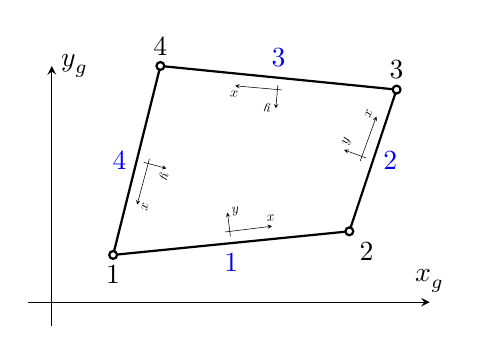
\begin{tikzpicture}[scale=6,>=stealth]
 \tikzstyle{elemnode} = [draw,circle,inner sep=1,fill=white]
 \newcommand{\lcoordsys}[2]{
   \begin{scope}[transform canvas={shift={#2},scale=0.5,rotate=#1}]
    \draw[->] (0,0.05) ++(-0.02,0) -- ++(0.2,0) node[above] {$x$};
    \draw[->] (0,0.05) ++(0,-0.02) -- ++(0,0.1) node[right] {$y$};
   \end{scope}
 }

 \draw[->] (-0.05,0) -- (0.8,0) node[above] {$x_g$};
 \draw[->] (0,-0.05) -- (0,0.5) node[right] {$y_g$};
 
 \draw[thick,xshift=-2] 
     (0.2,0.1)
  -- (0.7,0.15) coordinate[midway] (e1) node[below,midway,blue] {1} node[elemnode] {} node[below right] {2}
  -- (0.8,0.45) coordinate[midway] (e2) node[right,midway,blue] {2} node[elemnode] {} node[above] {3}
  -- (0.3,0.5)  coordinate[midway] (e3) node[above,midway,blue] {3} node[elemnode] {} node[above] {4}
  -- (0.2,0.1)  coordinate[midway] (e4) node[left,midway,blue] {4} node[elemnode] {} node[below] {1};

 \lcoordsys{  7}{(e1)};
 \lcoordsys{ 70}{(e2)};
 \lcoordsys{175}{(e3)};
 \lcoordsys{255}{(e4)};
\end{tikzpicture}

 \end{makeimage}
 \caption{PlaneStress2d element. Node numbering, edge numbering and definition of local edge c.s.(a).}
 \label{Planestress2dfig}
\end{figure}

\begin{elementsummary}{planestress2d}{2D quadrilateral element for plane stress analysis}{\optField{NIP}{in}}{planestress2d element summary}{planestress2dsummary}
\elementParam{\param{NIP}: allows to set the number of integration points}
\elementDescription{Unknowns}{Two dofs (u-displacement, v-displacement) are required in each node.}
\elementDescription{Approximation}{Linear approximation of displacements and geometry.}
\elementDescription{Integration}{Integration of membrane strain terms using Gauss integration formula in 1, 4 (default), 9 or 16 integration points. The default number of integration points used can be overloaded using \param{NIP} parameter. Reduced integration for shear terms is employed. Shear terms are always integrated using the 1-point integration rule.}
\elementDescription{Features}{Nonlocal constitutive support, Geometric nonlinearity support.}
\elementDescription{CS properties}{cross section thickness is required.}
\elementDescription{Loads}{Body loads are supported. Boundary loads are supported and computed using numerical integration. The side numbering is following. Each i-th element side begins in i-th element node and ends on next element node (i+1-th node or 1-st node, in the case of side number 4). The local positive edge x-axis coincides with side direction, the positive local edge y-axis is rotated 90 degrees anti-clockwise (see fig. (\ref{Planestress2dfig})).}
\elementDescription{Nlgeo}{0, 1.}
\elementDescription{Status}{Reliable}
\end{elementsummary}

\subsubsection{QPlaneStress2d}

Implementation of quadratic isoparametric eight-node quadrilateral
plane-stress  finite element. Each node has 2 degrees of freedom.
The node numbering is anti-clockwise and is explained in fig. (\ref
{qplanstrssfig}). The element features are summarized in Table~\ref{qplanestress2dsummary}.

\begin{figure}[htb]
 \centering
 \begin{makeimage}
  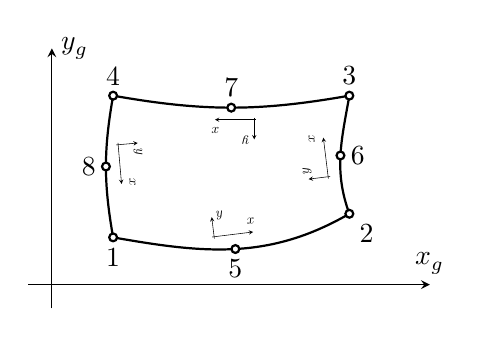
\begin{tikzpicture}[scale=6,>=stealth]
 \tikzstyle{elemnode} = [draw,circle,inner sep=1,fill=white]
\newcommand{\lcoordsys}[1]{\draw[->] (-0.05,0) -- (1,0) node[above] {$x_{#1}$}; \draw[->] (0,-0.05) -- (0,0.5) node[right] {$y_{#1}$};}
 \draw[->] (-0.05,0) -- (0.8,0) node[above] {$x_g$};
 \draw[->] (0,-0.05) -- (0,0.5) node[right] {$y_g$};
 
 \draw[thick,xshift=-2] 
     (0.2,0.1) node[elemnode] {} node[below] {1}
  to[out=-10,in=210] coordinate[midway] (e1) node[elemnode,midway] {} node[below,midway] {5} (0.7,0.15) node[elemnode] {} node[below right] {2}
  to[out=110,in=-100]  coordinate[midway] (e2)  node[elemnode,midway] {} node[right,midway] {6} (0.7,0.4) node[elemnode] {} node[above] {3}
  to[out=190,in=-10] coordinate[midway] (e3) node[elemnode,midway] {} node[above,midway] {7} (0.2,0.4) node[elemnode] {} node[above] {4}
  to[out=-100,in=100] coordinate[midway] (e4) node[elemnode,midway] {} node[left,midway] {8} (0.2,0.1);

\node[above] at (e1) {\rotatebox{7}{\scalebox{0.5}{\tikz{\lcoordsys{}}}}};
\node[left] at (e2) {\rotatebox{97}{\scalebox{0.5}{\tikz{\lcoordsys{}}}}};
\node[below] at (e3) {\rotatebox{180}{\scalebox{0.5}{\tikz{\lcoordsys{}}}}};
\node[right] at (e4) {\rotatebox{275}{\scalebox{0.5}{\tikz{\lcoordsys{}}}}};
\end{tikzpicture}

 \end{makeimage}
 \caption{QPlaneStress2d element - node numbering.}
 \label{qplanstrssfig}
\end{figure}

\begin{elementsummary}{qplanestress2d}{2D quadratic isoparametric plane stress element}{\optField{NIP}{in}}{qplanestress2d element summary}{qplanestress2dsummary}
\elementParam{\param{NIP}: allows to set the number of integration points}
\elementDescription{Unknowns}{Two dofs (u-displacement, v-displacement) are required in each node.}
\elementDescription{Approximation}{Quadratic approximation of displacements and geometry.}
\elementDescription{Integration}{Full integration using Gauss integration formula in 4 (the default), 9 or 16 integration points. The default number of integration points used can be overloaded using \param{NIP} parameter.}
\elementDescription{Features}{Adaptivity support.}
\elementDescription{CS properties}{Cross section thickness is required.}
\elementDescription{Loads}{Body and boundary loads are supported.}
\elementDescription{Nlgeo}{0, 1.}
\elementDescription{Status}{Stable}
\end{elementsummary}




\subsubsection{TrPlaneStress2d}
Implements an triangular three-node  constant strain plane-stress  
finite element. Each node has 2 degrees of freedom.
The node numbering is anti-clockwise. The element features are summarized in Table~\ref{trplanestress2dsummary}.

\begin{figure}[htb]
 \centering
 \begin{makeimage}
   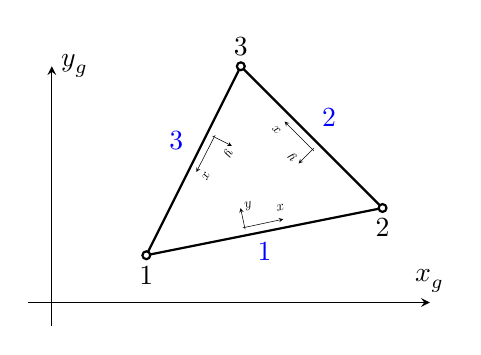
\begin{tikzpicture}[scale=6,>=stealth]
 \tikzstyle{elemnode} = [draw,circle,inner sep=1,fill=white]
 \newcommand{\lcoordsys}[1]{\draw[->] (-0.05,0) -- (1,0) node[above] {$x_{#1}$}; \draw[->] (0,-0.05) -- (0,0.5) node[right] {$y_{#1}$};}
 \draw[->] (-0.05,0) -- (0.8,0) node[above] {$x_g$};
 \draw[->] (0,-0.05) -- (0,0.5) node[right] {$y_g$};
 
 \draw[thick] 
     (0.2,0.1) node[elemnode] {} node[below] {1}
  -- (0.7,0.2) node[elemnode] {} node[below] {2} node[blue,midway,below] {1} coordinate[midway] (e1)
  -- (0.4,0.5) node[elemnode] {} node[above] {3} node[blue,midway,above right] {2} coordinate[midway] (e2)
  -- (0.2,0.1) node[blue,midway,above left] {3} coordinate[midway] (e3);

 \node[yshift=8] at (e1) {\rotatebox{12}{\scalebox{0.5}{\tikz{\lcoordsys{}}}}};
 \node[xshift=-9,yshift=-2] at (e2) {\rotatebox{135}{\scalebox{0.5}{\tikz{\lcoordsys{}}}}};
 \node[xshift=8,yshift=-1] at (e3) {\rotatebox{243}{\scalebox{0.5}{\tikz{\lcoordsys{}}}}};
\end{tikzpicture}

 \end{makeimage}
 \caption{TrPlaneStress2d element - node and side numbering.}
 \label{TrPlanestressfig}
\end{figure}

\begin{elementsummary}{trplanestress2d}{2D linear triangular isoparametric plane stress element}{-}{trplanestress2d element summary}{trplanestress2dsummary}
\elementDescription{Unknowns}{Two dofs (u-displacement, v-displacement) are required in each node.}
\elementDescription{Approximation}{Linear approximation of displacements and geometry.}
\elementDescription{Integration}{Integration of membrane strain terms using one point gauss integration formula.}
\elementDescription{Features}{Nonlocal constitutive support, Edge load support, Geometric nonlinearity support, Adaptivity support.}
\elementDescription{CS properties}{Cross section thickness is required.}
\elementDescription{Loads}{Body loads are supported. Boundary loads are
supported and are computed  using numerical integration. The side numbering is
following. Each i-th element side begins in i-th element node and
ends on next element node (i+1-th node or 1-st node, in the case of 
side number 3). The local positive edge x-axis coincides with side
direction, the positive local edge y-axis is rotated 90 degrees
anti-clockwise (see fig. (\ref{TrPlanestressfig})).}
\elementDescription{Nlgeo}{0, 1.}
\elementDescription{Status}{Reliable}
\end{elementsummary}



\subsubsection{QTrPlStr}
Implementation of quadratic six-node plane-stress finite
element. Each node has 2 degrees of freedom. Node numbering is
anti-clockwise and is shown in fig. (\ref{qtrplanstressfig}). The element features are summarized in Table~\ref{qtrplstrsummary}.

\begin{figure}[htb]
 \centering
 \begin{makeimage}
  \tikzstyle{elemnode} = [draw,circle,inner sep=1,fill=white]
\begin{tikzpicture}[scale=6,>=stealth]
 \draw[->] (-0.05,0) -- (0.8,0) node[above] {$x$};
 \draw[->] (0,-0.05) -- (0,0.5) node[right] {$y$};
 
 \draw[thick,xshift=-2] 
     (0.2,0.1) node[elemnode] {} node[below] {1}
  to[out=-10,in=210] node[elemnode,midway] {} node[below,midway] {4} (0.7,0.2) node[elemnode] {} node[below right] {2}
  to[out=110,in=-20] node[elemnode,midway] {} node[above right,midway] {5} (0.4,0.5) node[elemnode] {} node[above] {3}
  to[out=-90,in=40] node[elemnode,midway] {} node[above left,midway] {6} (0.2,0.1);
\end{tikzpicture}

 \end{makeimage}
 \caption{QTrPlStr element - node and side numbering.}
 \label{qtrplanstressfig}
\end{figure}

\begin{elementsummary}{qtrplstr}{2D quadratic triangular plane stress element}{\optField{NIP}{in}}{qtrplstr element summary}{qtrplstrsummary}
\elementParam{\param{NIP}: allows to set the number of integration points}
\elementDescription{Unknowns}{Two dofs (u-displacement, v-displacement) are required in each node.}
\elementDescription{Approximation}{Quadratic approximation of displacements and geometry.}
\elementDescription{Integration}{Full integration using gauss integration formula in 4 points (the
default) or in 7 points (using \param{NIP} parameter).}
\elementDescription{Features}{Adaptivity support (error indicator).}
\elementDescription{CS properties}{Cross section thickness is required.}
\elementDescription{Loads}{Boundary loads are supported.}
\elementDescription{Nlgeo}{0, 1.}
\elementDescription{Status}{-}
\end{elementsummary}




\subsubsection{TrPlaneStrRot}
Implementation of triangular three-node  plane-stress 
finite element with independent rotation field.
Each node has 3 degrees of freedom. The element features are summarized in Table~\ref{trplanestrrotsummary}.
The implementation is based on the following paper: Ibrahimbegovic, A., Taylor, R.L., Wilson, E. L.: A robust membrane qudritelar element with rotational degrees of freedom, Int. J. Num. Meth. Engng., 30, 445-457, 1990.
The rotation field is defined as $\omega = \del{1}{2}(\der{v}{x}-\der{u}{y}) = \nabla_u\mbf{u}$. The following form of potential energy functial is assumed:
\begin{equation*}
\Pi = \del{1}{2}\int_{\Omega}\mbf{\sigma}^T\mbf{\varepsilon}\ d\Omega + \int_{\Omega}\mbf{\tau}^T(\nabla_u\mbf{u}-\omega)\ d\Omega - \int_\Omega \mbf{X}^T\mbf{u}\ d\Omega
\end{equation*}
where $\mbf{\tau}$ is pseudo-stress (component of anti-symmetric stress tensor) working on dislocation $(\nabla_u\mbf{u}-\omega)$; the following constitutive relation foris assumed: $\mbf{\tau} = G(\nabla_u\mbf{u}-\omega)$, where $G$ is elasticity modulus in shear.

\begin{elementsummary}{trplanestrrot}{2D linear triangular plane stress element with rotational DOFs}{\optField{NIP}{in} \optField{NIPRot}{in}}{trplanestrrot element summary}{trplanestrrotsummary}
\elementParam{\param{NIP}: allows to set the number of integration points for integration of membrane terms.}
\elementParam{\param{NIPRot}: allows to set the number of integration points for integration of terms associated to rotational field.}
\elementDescription{Unknowns}{Three dofs (u-displacement, v-displacement, z-rotation) are required in each node.}
\elementDescription{Approximation}{Linear approximation of displacements and geometry.}
\elementDescription{Integration}{Integration of membrane strain terms using gauss integration formula in 4 points (default) or using 1 or 7 points (using \param{NIP} parameter). Integration of strains associated with rotational field integration using 1 point is default (4 and 7 points rules can be specified using \param{NIPRot} parameter).}
\elementDescription{Features}{-}
\elementDescription{CS properties}{Cross section thickness is required.}
\elementDescription{Loads}{-}
\elementDescription{Nlgeo}{0.}
\elementDescription{Status}{-}
\end{elementsummary}

\subsubsection{TrPlaneStressRotAllman}
Implementation of triangular three-node  plane-stress 
with nodal rotations.
Each node has 3 degrees of freedom. The element features are summarized in Table~\ref{TrPlaneStressRotAllmansummary}.
The implementation is based on the following paper: Allman, D.J.: A compatible triangular element including vertex rotations for plane elasticity analysis, Computers \& Structures, vol. 19, no. 1-2, pp. 1-8, 1984.
The element is based on plane stress element with quadratic interpolation. The displacements in midside nodes are expressed using vertex displacements and vertex rotations (for edge normal displacement component); the tangential component is interpolated from vertex values. For particular element side starting at i-th vertex and ending in j-th vertex the normal and tangential displacements at edge midpoint can be expressed as
\begin{eqnarray*}
u_n\vert_{l/2} &=& \del{u_{ni}+u_{nj}}{2}+\del{l}{8}(\omega_i-\omega_j)\\
u_t\vert_{l/2} &=& \del{u_{ti}+u_{tj}}{2}
\end{eqnarray*}
where $l$ is edge length. This allows to express global displacements in element midside nodes using vertex displacements and rotations. For a single edge, one obtains:
\begin{eqnarray*}
u\vert_{l/2} &=&-\del{u_{ni}+u_{nj}}{2}+\del{l}{8}(\omega_i-\omega_j)\del{\Delta y_{ji}}{l}+(\del{u_{t1}+u_{t2}}{2})\del{\Delta x_{ji}}{l}\\
v\vert_{l/2} &=& \del{u_{ni}+u_{nj}}{2}+\del{l}{8}(\omega_i-\omega_j)\del{\Delta x_{ji}}{l}+(\del{u_{t1}+u_{t2}}{2})\del{\Delta y_{ji}}{l}\\
\end{eqnarray*}

\begin{elementsummary}{trplanestressrotallman}{2D linear triangular plane stress element with rotational DOFs}{}{trplanestressrotallman element summary}{TrPlaneStressRotAllmansummary}
\elementDescription{Unknowns}{Three dofs (u-displacement, v-displacement, z-rotation) are required in each node.}
\elementDescription{Approximation}{Linear approximation of geometry, quadratic interpolation of displacements.}
\elementDescription{Integration}{Integration of membrane strain terms using gauss integration formula in 4 points.}
\elementDescription{Zero energy mode}{The zero energy mode (equal rotations) is handled by adding additional energy term preventing spurious modes.}

\elementDescription{Features}{-}
\elementDescription{CS properties}{Cross section thickness is required.}
\elementDescription{Loads}{-}
\elementDescription{Nlgeo}{0.}
\elementDescription{Status}{-}
\end{elementsummary}



%-----------------------------------------------------------------------------------------------
\clearpage
\subsection{Plane Strain Elements}

\subsubsection{Quad1PlaneStrain}
Represents isoparametric four-node quadrilateral plane-strain
finite element. Each node has 2 degrees of freedom.
Structure should be defined in x,y plane. 
The nodes should be numbered anti-clockwise (positive rotation around
z-axis). The element features are summarized in Table~\ref{quad1planestrainsummary}.

\begin{figure}[htb]
 \centering
 \begin{makeimage}
  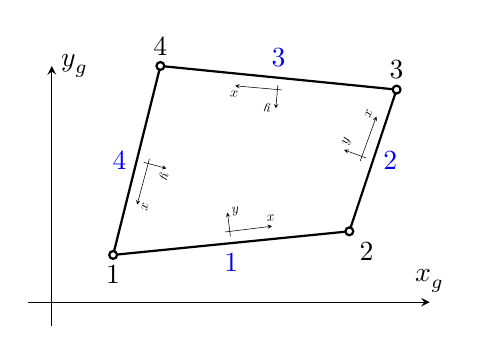
\begin{tikzpicture}[scale=6,>=stealth]
 \tikzstyle{elemnode} = [draw,circle,inner sep=1,fill=white]
 \newcommand{\lcoordsys}[2]{
   \begin{scope}[transform canvas={shift={#2},scale=0.5,rotate=#1}]
    \draw[->] (0,0.05) ++(-0.02,0) -- ++(0.2,0) node[above] {$x$};
    \draw[->] (0,0.05) ++(0,-0.02) -- ++(0,0.1) node[right] {$y$};
   \end{scope}
 }

 \draw[->] (-0.05,0) -- (0.8,0) node[above] {$x_g$};
 \draw[->] (0,-0.05) -- (0,0.5) node[right] {$y_g$};
 
 \draw[thick,xshift=-2] 
     (0.2,0.1)
  -- (0.7,0.15) coordinate[midway] (e1) node[below,midway,blue] {1} node[elemnode] {} node[below right] {2}
  -- (0.8,0.45) coordinate[midway] (e2) node[right,midway,blue] {2} node[elemnode] {} node[above] {3}
  -- (0.3,0.5)  coordinate[midway] (e3) node[above,midway,blue] {3} node[elemnode] {} node[above] {4}
  -- (0.2,0.1)  coordinate[midway] (e4) node[left,midway,blue] {4} node[elemnode] {} node[below] {1};

 \lcoordsys{  7}{(e1)};
 \lcoordsys{ 70}{(e2)};
 \lcoordsys{175}{(e3)};
 \lcoordsys{255}{(e4)};
\end{tikzpicture}

 \end{makeimage}
 \caption{Quad1PlaneStrain element. Node numbering, Side numbering and
 definition of local edge c.s.(a).}
 \label{Quad1PlaneStrainfig}
\end{figure}

\begin{elementsummary}{quad1planestrain}{2D linear quadrilateral plane-strain element}{\optField{NIP}{in}}{quad1planestrain element summary}{quad1planestrainsummary}
\elementParam{\param{NIP}: allows to set the number of integration points for integration of membrane terms.}
\elementDescription{Unknowns}{Two dofs (u-displacement, v-displacement) are required in each node.}
\elementDescription{Approximation}{Linear approximation of displacements and geometry.}
\elementDescription{Integration}{Integration of membrane strain terms using gauss integration formula in 4 (the default), 9 or 16 integration points. The default number of integration points used can be overloaded using \param{NIP} parameter. Reduced integration for shear terms is employed. Shear terms are always integrated using 1 point integration rule.}
\elementDescription{Features}{Nonlocal constitutive support, Adaptivity support.}
\elementDescription{CS properties}{Cross section thickness is required.}
\elementDescription{Loads}{Body loads are supported. Boundary loads are supported and computed using numerical integration. The side numbering is following. Each i-th element side begins in i-th element node and ends on next element node (i+1-th node or 1-st node, in the case of side number 4). The local positive edge x-axis coincides with side direction, the positive local edge y-axis is rotated 90 degrees anti-clockwise (see fig. (\ref{Quad1PlaneStrainfig})).}
\elementDescription{Nlgeo}{0.}
\elementDescription{Status}{Reliable}
\end{elementsummary}





\subsubsection{TrplaneStrain}
Implements an triangular three-node  constant strain plane-strain  
finite element. Each node has 2 degrees of freedom.
The node numbering is anti-clockwise. The element features are summarized in Table~\ref{trplanestrainsummary}.

\begin{figure}[htb]
 \centering
 \begin{makeimage}
  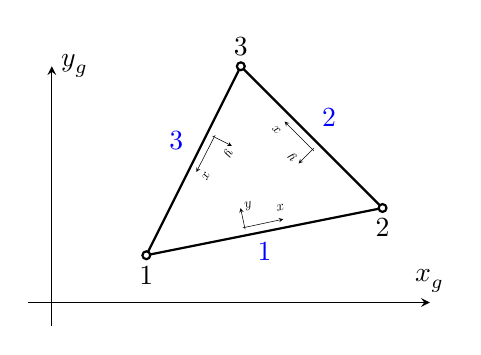
\begin{tikzpicture}[scale=6,>=stealth]
 \tikzstyle{elemnode} = [draw,circle,inner sep=1,fill=white]
 \newcommand{\lcoordsys}[1]{\draw[->] (-0.05,0) -- (1,0) node[above] {$x_{#1}$}; \draw[->] (0,-0.05) -- (0,0.5) node[right] {$y_{#1}$};}
 \draw[->] (-0.05,0) -- (0.8,0) node[above] {$x_g$};
 \draw[->] (0,-0.05) -- (0,0.5) node[right] {$y_g$};
 
 \draw[thick] 
     (0.2,0.1) node[elemnode] {} node[below] {1}
  -- (0.7,0.2) node[elemnode] {} node[below] {2} node[blue,midway,below] {1} coordinate[midway] (e1)
  -- (0.4,0.5) node[elemnode] {} node[above] {3} node[blue,midway,above right] {2} coordinate[midway] (e2)
  -- (0.2,0.1) node[blue,midway,above left] {3} coordinate[midway] (e3);

 \node[yshift=8] at (e1) {\rotatebox{12}{\scalebox{0.5}{\tikz{\lcoordsys{}}}}};
 \node[xshift=-9,yshift=-2] at (e2) {\rotatebox{135}{\scalebox{0.5}{\tikz{\lcoordsys{}}}}};
 \node[xshift=8,yshift=-1] at (e3) {\rotatebox{243}{\scalebox{0.5}{\tikz{\lcoordsys{}}}}};
\end{tikzpicture}
 % Same image for plane stress
 \end{makeimage}
 \caption{TrplaneStrain element - node and side numbering.}
 \label{TrplaneStrain}
\end{figure}

\begin{elementsummary}{trplanestrain}{2D linear triangular plane-strain element}{-}{trplanestrain element summary}{trplanestrainsummary}
%\elementParam{\param{NIP}: allows to set the number of integration points for integration of membrane terms.}
\elementDescription{Unknowns}{Two dofs (u-displacement, v-displacement) are required in each node.}
\elementDescription{Approximation}{Linear approximation of displacements and geometry.}
\elementDescription{Integration}{Integration of membrane strain terms using one point gauss integration formula.}
\elementDescription{Features}{Nonlocal constitutive support. Edge load support, Adaptivity support.}
\elementDescription{CS properties}{Cross section thickness is required.}
\elementDescription{Loads}{Body loads are supported. Boundary loads are supported and are computed  using numerical integration. The side numbering is following. Each i-th element side begins in i-th element node and ends on next element node (i+1-th node or 1-st node, in the case of side number 3). The local positive edge x-axis coincides with side direction, the positive local edge y-axis is rotated 90 degrees anti-clockwise (see fig. (\ref{TrplaneStrain})).}
\elementDescription{Nlgeo}{0.}
\elementDescription{Status}{Reliable}
\end{elementsummary}




%-----------------------------------------------------------------------------------------------
\clearpage
\subsection{Plate\&Shell Elements}
\subsubsection {CCT Element}
\label{cct}
Implementation of constant curvature triangular element for plate
analysis. Formulation based on Mindlin hypothesis. The structure should be defined in x,y plane. 
The nodes should be numbered anti-clockwise (positive rotation around
z-axis). The element features are summarized in Table~\ref{cctplatesummary}.


\begin{elementsummary}{cctplate}{2D constant curvature triangular plate element}{-}{cctplate element summary}{cctplatesummary}
%\elementParam{\param{NIP}: allows to set the number of integration points for integration of membrane terms.}
\elementDescription{Unknowns}{Three dofs (w-displacement, u and v - rotations) are required in each node.}
\elementDescription{Approximation}{Linear approximation of ratations, quadratic approximation of displacement.}
\elementDescription{Integration}{Integration of all terms using one point formula.}
\elementDescription{Features}{Layered cross section support.}
\elementDescription{CS properties}{Cross section thickness is required.}
\elementDescription{Loads}{Body loads are supported. Boundary loads are not supported now.}
\elementDescription{Output}{On output, the generalized strains are printed in a vector with 12 components, with the following meaning:
$$e=\{\varepsilon_x, \varepsilon_y, \varepsilon_z, \gamma_{yz}, \gamma_{zx}, \gamma_{xy}, \kappa_x, \kappa_y, \kappa_z, \kappa_{yz}, \kappa_{xz}, \kappa_{xy}\},$$where $\varepsilon_x, \varepsilon_y, \varepsilon_z$ are membrane normal deformations, $\gamma_{yz}, \gamma_{zx}, \gamma_{xy}$ are shear componets, and $\kappa_x, \kappa_y, \kappa_z, \kappa_{yz}, \kappa_{xz}, \kappa_{xy}$ are curvatures.
The generalized stress vector contains corresponding integral forces/moments:
$$s=\{n_x, n_y, n_y, v_{yz}, v_{zx}, v_{xy}, m_x, m_y, m_z, m_{yz}, m_{xz}, m_{xy}\}.$$ Please note, for example, that bending moment $m_x$ is defined as $m_x=\int \sigma_x z\ dz$, so it acts along the y-axis and positive value causes tension in bottom layer.}
\elementDescription{Nlgeo}{0.}
\elementDescription{Status}{Reliable}
\end{elementsummary}






\subsubsection {CCT3D Element}
Implementation of constant curvature triangular element for plate
analysis. Formulation based on Mindlin hypothesis. The element could be arbitrarily oriented in space. 
The nodes should be numbered anti-clockwise (positive rotation around element normal). 
The element features are summarized in Table~\ref{cctplate3dsummary}.

\begin{elementsummary}{cctplate3d}{Constant curvature triangular plate element in arbitray position}{-}{cctplate3d element summary}{cctplate3dsummary}
%\elementParam{\param{NIP}: allows to set the number of integration points for integration of membrane terms.}
\elementDescription{Unknowns}{Six dofs (u,v,w-displacements and u,v,w rotations) are in general required in each node.}
\elementDescription{Approximation}{Linear approximation of ratations, quadratic approximation of displacement.}
\elementDescription{Integration}{Integration of all terms using one point formula.}
\elementDescription{Features}{Layered cross section support.}
\elementDescription{CS properties}{Cross section thickness is required.}
\elementDescription{Loads}{Body loads are supported. Boundary loads are not supported now.}
\elementDescription{Output}{On output, the generalized strains are printed in a vector with 12 components, with the following meaning:
$$e=\{\varepsilon_x, \varepsilon_y, \varepsilon_z, \gamma_{yz}, \gamma_{zx}, \gamma_{xy}, \kappa_x, \kappa_y, \kappa_z, \kappa_{yz}, \kappa_{xz}, \kappa_{xy}\},$$where $\varepsilon_x, \varepsilon_y, \varepsilon_z$ are membrane normal deformations, $\gamma_{yz}, \gamma_{zx}, \gamma_{xy}$ are shear componets, and $\kappa_x, \kappa_y, \kappa_z, \kappa_{yz}, \kappa_{xz}, \kappa_{xy}$ are curvatures.
The generalized stress vector contains corresponding integral forces/moments:
$$s=\{n_x, n_y, n_y, v_{yz}, v_{zx}, v_{xy}, m_x, m_y, m_z, m_{yz}, m_{xz}, m_{xy}\}.$$ Please note, for example, that bending moment $m_x$ is defined as $m_x=\int \sigma_x z\ dz$, so it acts along the y-axis and positive value causes tension in bottom layer.}
\elementDescription{Nlgeo}{0.}
\elementDescription{Status}{Reliable}
\end{elementsummary}


\subsubsection {RerShell Element}
Combination of CCT plate element (Mindlin hypothesis) with triangular plane stress element
for membrane behavior. The element curvature can be specified. 
Although element requires generally six DOFs per node, no stiffness to
local rotation along z-axis (rotation around element normal) is supplied. 
The element features are summarized in Table~\ref{rershellsummary}.

\begin{elementsummary}{rershell}{Simple shell based on combination of CCT plate element (Mindlin hypothesis) with triangular plane stress element. element can be arbitrary positioned in space.}{-}{rershell element summary}{rershellsummary}
%\elementParam{\param{NIP}: allows to set the number of integration points for integration of membrane terms.}
\elementDescription{Unknowns}{Six dofs (u,v,w-displacements and u,v,w rotations) are in general required in each node. Note, that although element it requires generally six DOFs per node, no stiffness to local rotation along z-axis (rotation around element normal) is supplied.}
\elementDescription{Approximation}{Linear approximation of ratations, quadratic approximation of displacement.}
\elementDescription{Integration}{Integration of all terms using one point formula.}
\elementDescription{Features}{Layered cross section support.}
\elementDescription{CS properties}{Cross section thickness is required.}
\elementDescription{Loads}{Body loads are supported. Boundary loads are not supported now.}
\elementDescription{Output}{On output, the generalized strains are printed in a vector with 12 components, with the following meaning:
$$e=\{\varepsilon_x, \varepsilon_y, \varepsilon_z, \gamma_{yz}, \gamma_{zx}, \gamma_{xy}, \kappa_x, \kappa_y, \kappa_z, \kappa_{yz}, \kappa_{xz}, \kappa_{xy}\},$$where $\varepsilon_x, \varepsilon_y, \varepsilon_z$ are membrane normal deformations, $\gamma_{yz}, \gamma_{zx}, \gamma_{xy}$ are shear componets, and $\kappa_x, \kappa_y, \kappa_z, \kappa_{yz}, \kappa_{xz}, \kappa_{xy}$ are curvatures.
The generalized stress vector contains corresponding integral forces/moments:
$$s=\{n_x, n_y, n_y, v_{yz}, v_{zx}, v_{xy}, m_x, m_y, m_z, m_{yz}, m_{xz}, m_{xy}\}.$$ Please note, for example, that bending moment $m_x$ is defined as $m_x=\int \sigma_x z\ dz$, so it acts along the y-axis and positive value causes tension in bottom layer.}
\elementDescription{Nlgeo}{0.}
\elementDescription{Status}{Reliable}
\end{elementsummary}



\subsubsection {tr\_shell01 element}
Combination of CCT3D plate element (Mindlin hypothesis) with triangular plane stress element
for membrane behavior. It comes with complete set of 6 DOFs per node. 
The element features are summarized in Table~\ref{trshell01summary}.
\begin{figure}[htb]
 \centering
 \begin{makeimage}
  \tikzstyle{elemnode} = [solid,draw,thin,circle,inner sep=1,fill=white]

\begin{tikzpicture}[scale=6,>=stealth,
  x={(1cm,0cm)}, y={(0.5cm,0.5cm)}, z={(0cm,1cm)}]
 
 \begin{scope}
 \draw[->] (-0.05,0,0) -- (0.5,0,0) node[at end, below] {$x_g$};
 \draw[->] (0,-0.05,0) -- (0,0.5,0) node[at end, below right] {$y_g$};
 \draw[->] (0,0,-0.05) -- (0,0,0.5) node[at end, right] {$z_g$};
 \end{scope}

 \draw[very thick,-]
    (0.50, 0.10, 0.25) node[elemnode] {} node[below left] {1} -- node[midway, blue, below right] {1}
    (1.00, 0.25, 0.25) node[elemnode] {} node[right] {2}      -- node[near end, blue, above] {2}
    (0.10, 0.30, 0.50) node[elemnode] {} node[above left] {3} -- node[midway, blue, below left] {3}
    (0.50, 0.10, 0.25);

 % Shadow helps to visualize the depth
 \fill[fill=black!10]
    (0.50, 0.10, 0.) -- 
    (1.00, 0.25, 0.) -- 
    (0.10, 0.30, 0.) -- 
    (0.50, 0.10, 0.);

 % Draw normal (using latex arrow head, looks nicest)
 \draw[-latex] (0.5333,0.22, 0.33) -- +(0.1,-0.125,0.25) node[below right] {$\mathbf{n}$};
 
\end{tikzpicture}
 \end{makeimage}
 \caption{Geometry of tr\_shell01 element.}
\end{figure}

\begin{elementsummary}{tr\_shell01}{Triangular shell element combining CCT3D plate element (Mindlin hypothesis) with triangular plane stress element with rotational DOFs}{-}{tr\_shell01 element summary}{trshell01summary}
%\elementParam{\param{NIP}: allows to set the number of integration points for integration of membrane terms.}
\elementDescription{Unknowns}{Six dofs (u,v,w-displacements and u,v,w rotations) are in general required in each node.}
\elementDescription{Approximation}{See description of cct and trplanstrrot elements}
\elementDescription{Integration}{Integration of all terms using one point formula.}
\elementDescription{Features}{Layered cross section support.}
\elementDescription{CS properties}{Cross section thickness is required.}
\elementDescription{Loads}{Body loads are supported. Boundary loads are not supported now.}
\elementDescription{Output}{On output, the generalized strains are printed in a vector with 12 components, with the following meaning:
$$e=\{\varepsilon_x, \varepsilon_y, \varepsilon_z, \gamma_{yz}, \gamma_{zx}, \gamma_{xy}, \kappa_x, \kappa_y, \kappa_z, \kappa_{yz}, \kappa_{xz}, \kappa_{xy}\},$$where $\varepsilon_x, \varepsilon_y, \varepsilon_z$ are membrane normal deformations, $\gamma_{yz}, \gamma_{zx}, \gamma_{xy}$ are shear componets, and $\kappa_x, \kappa_y, \kappa_z, \kappa_{yz}, \kappa_{xz}, \kappa_{xy}$ are curvatures.
The generalized stress vector contains corresponding integral forces/moments:
$$s=\{n_x, n_y, n_y, v_{yz}, v_{zx}, v_{xy}, m_x, m_y, m_z, m_{yz}, m_{xz}, m_{xy}\}.$$ Please note, for example, that bending moment $m_x$ is defined as $m_x=\int \sigma_x z\ dz$, so it acts along the y-axis and positive value causes tension in bottom layer.}
\elementDescription{Nlgeo}{0.}
\elementDescription{Status}{Reliable}
\end{elementsummary}


\subsubsection{Quad1Mindlin Element} \label{quad1mindlin}
This class implements an quadrilateral, bilinear, four-node Mindlin plate.
This type of element exhibit strong shear locking (thin plates exhibit almost no bending).
Implements the lumped mass matrix. The element features are summarized in Table~\ref{quad1mindlinsummary}.

\begin{elementsummary}{quad1mindlin}{Quadrilateral, bilinear, four-node Mindlin plate}{\optField{NIP}{in}}{quad1mindlin element summary}{quad1mindlinsummary}
%\elementParam{\param{NIP}: allows to set the number of integration points for integration of membrane terms.}
\elementDescription{Unknowns}{Three dofs (w-displacement, u and v - rotation) are required in each node.}
\elementDescription{Approximation}{Linear for all unknowns.}
\elementDescription{Integration}{Default uses 4 integration points. No reduced integration is used, as it causes numerical problems.}
\elementDescription{Features}{Layered cross section support.}
\elementDescription{CS properties}{Cross section thickness is required.}
\elementDescription{Loads}{Dead weight loads, and edge loads are supported.}
\elementDescription{Nlgeo}{0.}
\elementDescription{Reference}{\cite{RobertCook1989}}
\elementDescription{Status}{Experimental}
\end{elementsummary}



%-----------------------------------------------------------------------------------------------
\clearpage
\subsection{Axisymmetric Elements}
Implementation relies on elements located exclusively in $x,y$ plane. The coordinate $x$ corresponds to radius, $y$ is the axis of rotation. Approximation of displacement functions $u,v$ is carried out on a particular finite element. Nonzero strains read
\begin{eqnarray}
\varepsilon_{x}=\varepsilon_{r}&=&\frac{\partial u}{\partial x}\\
\varepsilon_{y}=\varepsilon_{z}&=&\frac{\partial v}{\partial y}\\
\varepsilon_{\theta}&=&\frac{u}{r}\\
\gamma_{xy}=\gamma_{rz}&=&\frac{\partial u}{\partial y} + \frac{\partial v}{\partial x}
\end{eqnarray}
Stress components can be computed from elasticity matrix. Note that this matrix corresponds to a submatrix of the full 3D elasticity matrix.
\begin{eqnarray}
\left\{\begin{array}{c} \sigma_x \\ \sigma_y \\ \sigma_\theta \\ \sigma_{xy} \end{array} \right\} = 
\frac{E}{(1+\nu)(1-2\nu)}\left[ \begin{array}{cccc} 1-\nu & \nu & \nu & 0 \\ \nu & 1-\nu & \nu & 0 \\ \nu & \nu & 1-\nu & 0 \\ 0 & 0 & 0 & (1-2\nu)/2 \end{array} \right] = 
\left\{\begin{array}{c} \varepsilon_x \\ \varepsilon_y \\ \varepsilon_\theta \\ \gamma_{xy} \end{array} \right\} 
\end{eqnarray}
In OOFEM, the strain vector is arranged as $\{\varepsilon_{x}, \varepsilon_{y}, \varepsilon_{\theta}, 0, 0, \gamma_{xy}\}^T$ and the stress vector $\{\sigma_{x}, \sigma_{y}, \sigma_{\theta}, 0, 0, \tau_{xy}\}^T$. Implementation assumes a segment of 1 rad.

\subsubsection{Axisymm3d element}
Implementation of triangular three-node finite element 
for axisymmetric continuum. Each node has 2 degrees of freedom. 
Node numbering and edge position is the same as in Fig.~\ref{TrPlanestressfig}. 
The element features are summarized in Table~\ref{axisymm3dsummary}. 

\begin{elementsummary}{Axisymm3d}{Triangular axisymmetric linear element}{\optField{NIP}{in} \optField{NIPfish}{in}}{Axisymm3d element summary}{axisymm3dsummary}
\elementParam{\param{NIP}: allows to set the number of integration points for integration of terms corresponding to $\varepsilon_x$ and $\varepsilon_y$ strains (possible completions are 1 (default), 4 and 7 point integration rule).}
\elementParam{\param{NIPfish}: allows to set the number of integration points for integration of remain terms (corresponding to $\varepsilon_\theta$ and
$\gamma_{rz}$) (Supported values include 1 (default)).}
\elementDescription{Unknowns}{Two dofs (u-displacement, v-displacement) are required in each node.}
\elementDescription{Approximation}{Linear approximation of displacement and geometry.}
\elementDescription{Integration}{The integration of $\varepsilon_x$ and $\varepsilon_y$ strains can be altered using
\param{NIP} paramter (default is 1 point integration).  The remaining terms corresponding to strain components $\varepsilon_\theta$ and
$\gamma_{rz}$ are by default evaluated at 1 integration point, this can be changed by \param{NIPfish} parameter.}
\elementDescription{Features}{-}
\elementDescription{CS properties}{-}
\elementDescription{Loads}{Boundary and body loads are supported.}
\elementDescription{Nlgeo}{0.}
\elementDescription{Status}{-}
\end{elementsummary}

\subsubsection{Q4axisymm element}
Implementation of quadratic isoparametric eight-node quadrilateral -
finite element for axisymmetric 3d continuum. 
Each node has 2 degrees of freedom. The element features are summarized in Table~\ref{q4axisymmsummary}.

\begin{elementsummary}{Q4axisymm}{Quadratic isoparametric eight-node quadrilateral for axisymmetric analysis}{\optField{NIP}{in} \optField{NIPfish}{in}}{Q4axisymm element summary}{q4axisymmsummary}
\elementParam{\param{NIP}: allows to set the number of integration points for integration of terms corresponding to $\varepsilon_x$ and $\varepsilon_y$ strains (possible completions are 1, 4 (default), 9, and 16).}
\elementParam{\param{NIPfish}: allows to set the number of integration points for integration of remain terms (corresponding to $\varepsilon_\theta$ and
$\gamma_{rz}$) (Supported values include 1 (default), 4, 9, and 16 integration point formula).}
\elementDescription{Unknowns}{Two dofs (u-displacement, v-displacement) are required in each node.}
\elementDescription{Approximation}{Quadratic approximation of displacement and geometry.}
\elementDescription{Integration}{The integration of terms corresponding to $\varepsilon_x$ and $\varepsilon_y$ strains can be altered using \param{NIP} parameter (default is 4 point formula). The remaining terms (creesponding to $\varepsilon_\theta$ and $\gamma_{rz}$) are integrated by default using 1 point formula (see \param{NIPfish} parameter).}
\elementDescription{Features}{-}
\elementDescription{CS properties}{-}
\elementDescription{Loads}{No boundary and body loads are supported.}
\elementDescription{Nlgeo}{0.}
\elementDescription{Status}{-}
\end{elementsummary}


\subsubsection{L4axisymm element}
Implementation of isoparametric four-node quadrilateral axisymmetric
finite element with linear interpolations of displacements $u, v$. Node numbering and edge position is the same as in Fig.~\ref{Planestress2dfig}. The element features are summarized in Table~\ref{l4axisymmsummary}.

\begin{elementsummary}{L4axisymm}{Isoparametric four-node quadrilateral element for axisymmetric analysis}{\optField{NIP}{in}}{L4axisymm element summary}{l4axisymmsummary}
\elementParam{\param{NIP}: allows to set the number of integration points for integration of terms corresponding to $\varepsilon_x$ and $\varepsilon_y$ strains (possible completions are 1, 4 (default), 9, and 16).}
\elementDescription{Unknowns}{Two dofs (u-displacement, v-displacement) are required in each node.}
\elementDescription{Approximation}{Linear approximation of displacement and geometry.}
\elementDescription{Integration}{The integration of $\varepsilon_x$ and $\varepsilon_y$ strains can be altered using
\param{NIP} parameter (possible completions are 1, 4 (default), 9 or 16
point integration rule). The remaining strain components ($\varepsilon_\theta$ and
$\gamma_{rz}$) are integrated using one point integration formula.}
\elementDescription{Features}{-}
\elementDescription{CS properties}{-}
\elementDescription{Loads}{Boundary and body loads supported.}
\elementDescription{Nlgeo}{0.}
\elementDescription{Status}{-}
\end{elementsummary}

%-----------------------------------------------------------------------------------------------
\clearpage
\subsection{3d Continuum Elements}
\subsubsection{LSpace element}
\label{lspacesect}
Implementation of Linear 3d  eight - node 
finite element. Each node has 3 degrees of freedom. The element features are summarized in Table~\ref{lspacesummary}.
\begin{figure}[htb]
 \centering
 \begin{makeimage}
  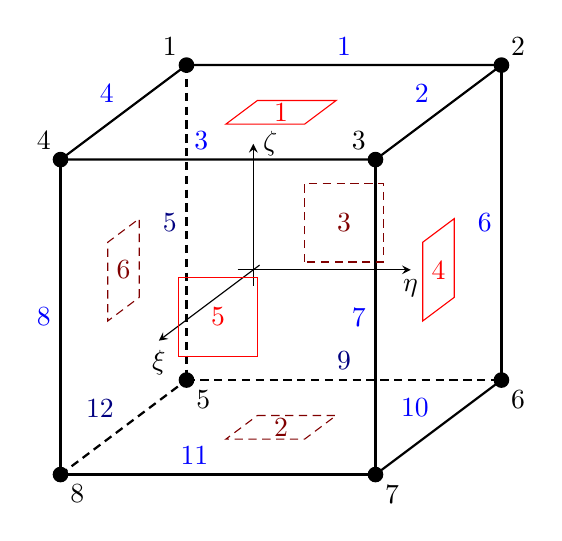
\begin{tikzpicture}[scale=2,>=stealth,
  x={(-0.4cm,-0.3cm)}, y={ (1cm,0cm) }, z={(0cm,1cm)}]
 \tikzstyle{elemnode} = [fill,circle,inner sep=2]
 \tikzstyle{background} = [densely dashed]
 \newcommand{\fs}{0.25}
 
% Coord.sys. (shifted for readability)
 \draw[->,xshift=-5] (-0.1,0,0) -- (1.5,0,0) node[at end,below] {$\xi$};
 \draw[->,xshift=-5] (0,-0.1,0) -- (0,1,0) node[at end,below] {$\eta$};
 \draw[->,xshift=-5] (0,0,-0.1) -- (0,0,0.8) node[at end,right] {$\zeta$};

% Can't use rectangle in 3d
 \draw[thick] (-1,-1,1) -- (-1,1,1) -- (1,1,1) -- (1,-1,1) -- cycle;
 \draw[thick,background] (-1,-1,-1) -- (-1,1,-1);
 \draw[thick] (-1,1,-1)-- (1,1,-1);
 \draw[thick] (1,1,-1) -- (1,-1,-1);
 \draw[thick,background] (1,-1,-1) -- (-1,-1,-1);
 \draw[thick,background] (-1,-1,1) -- (-1,-1,-1);
 \draw[thick] (-1,1,1) -- (-1,1,-1);
 \draw[thick] (1,-1,1) -- (1,-1,-1);
 \draw[thick] (1,1,1) -- (1,1,-1);

% Faces
 \draw[red] (1,-\fs,-\fs) -- (1,-\fs,\fs) -- (1,\fs,\fs) -- (1,\fs,-\fs) -- cycle;
 \node[red] at (1,0,0) {5};
 \draw[red] (-\fs,1,-\fs) -- (-\fs,1,\fs) -- (\fs,1,\fs) -- (\fs,1,-\fs) -- cycle;
 \node[red] at (0,1,0) {4};
 \draw[red] (-\fs,-\fs,1) -- (-\fs,\fs,1) -- (\fs,\fs,1) -- (\fs,-\fs,1) -- cycle;
 \node[red] at (0,0,1) {1};
 \draw[red!50!black,background] (-1,-\fs,-\fs) -- (-1,-\fs,\fs) -- (-1,\fs,\fs) -- (-1,\fs,-\fs) -- cycle;
 \node[red!50!black] at (-1,0,0) {3};
 \draw[red!50!black,background] (-\fs,-1,-\fs) -- (-\fs,-1,\fs) -- (\fs,-1,\fs) -- (\fs,-1,-\fs) -- cycle;
 \node[red!50!black] at (0,-1,0) {6};
 \draw[red!50!black,background] (-\fs,-\fs,-1) -- (-\fs,\fs,-1) -- (\fs,\fs,-1) -- (\fs,-\fs,-1) -- cycle;
 \node[red!50!black] at (0,0,-1) {2};

% Nodes
 \node[elemnode] (n1) at (-1,-1, 1) {}; \node[above left] at (n1) {1};
 \node[elemnode] (n2) at (-1, 1, 1) {}; \node[above right] at (n2) {2};
 \node[elemnode] (n3) at ( 1, 1, 1) {}; \node[above left] at (n3) {3};
 \node[elemnode] (n4) at ( 1,-1, 1) {}; \node[above left] at (n4) {4};
 \node[elemnode] (n5) at (-1,-1,-1) {}; \node[below right] at (n5) {5};
 \node[elemnode] (n6) at (-1, 1,-1) {}; \node[below right] at (n6) {6};
 \node[elemnode] (n7) at ( 1, 1,-1) {}; \node[below right] at (n7) {7};
 \node[elemnode] (n8) at ( 1,-1,-1) {}; \node[below right] at (n8) {8};

% Edges
 \node[blue,above] at (-1,0,1) {1};
 \node[blue,above left] at (0,1,1) {2};
 \node[blue,above left] at (1,0,1) {3};
 \node[blue,above left] at (0,-1,1) {4};

 \node[blue!50!black,left] at (-1,-1,0) {5};
 \node[blue,left] at (-1,1,0) {6};
 \node[blue,left] at (1,1,0) {7};
 \node[blue,left] at (1,-1,0) {8};

 \node[blue!50!black,above] at (-1,0,-1) {9};
 \node[blue,above left] at (0,1,-1) {10};
 \node[blue,above left] at (1,0,-1) {11};
 \node[blue!50!black,above left] at (0,-1,-1) {12};
\end{tikzpicture}

 \end{makeimage}
 \caption{LSpace element (Node numbers in black, side numbers in blue,
 and surface numbers in red).}
\end{figure}

\begin{elementsummary}{lspace}{Linear isoparametric brick element}{\optField{NIP}{in}}{lspace element summary}{lspacesummary}
\elementParam{\param{NIP}: allows to set the number of integration points (possible completions are 1, 8 (default), or 27).}
\elementDescription{Unknowns}{Three dofs (u-displacement, v-displacement, w-displacement) are required in each node.}
\elementDescription{Approximation}{Linear approximation of displacement and geometry.}
\elementDescription{Integration}{Full integration of all strain components.}
\elementDescription{Features}{Adaptivity support, Geometric nonlinearity support.}
\elementDescription{CS properties}{-}
\elementDescription{Loads}{-}
\elementDescription{Nlgeo}{0,1,2.}
\elementDescription{Status}{Reliable}
\end{elementsummary}


\subsubsection{LSpaceBB element}
Implementation of 3d brick eight - node 
linear approximation element with selective integration of deviatoric and volumetric 
strain contributions (B-bar formulation) for incompressible problems. 
Features and description identical to conventional lspace element, see section ~\ref{lspacesect}.

\subsubsection{QSpace element}\label{QSpace_element}
Implementation of quadratic 3d 20-node 
finite element. Each node has 3 degrees of freedom. The element features are summarized in Table~\ref{qspacesummary}.
\begin{figure}[htb]
 \centering
 \begin{makeimage}
  \raisebox{-0.5\height}{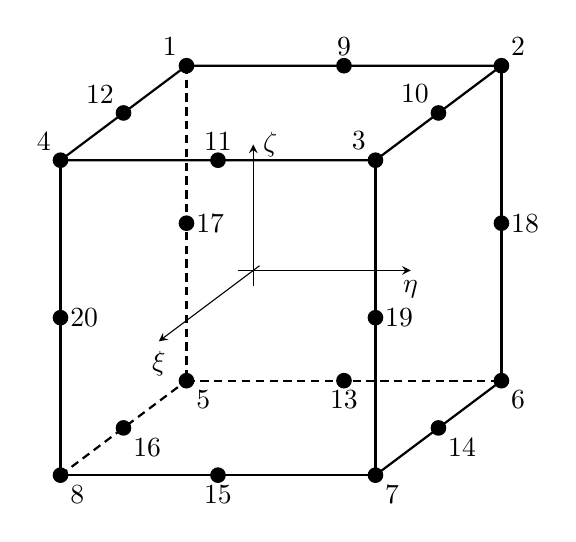
\begin{tikzpicture}[scale=2,>=stealth,
  x={(-0.4cm,-0.3cm)}, y={ (1cm,0cm) }, z={(0cm,1cm)}]
 \tikzstyle{elemnode} = [fill,circle,inner sep=2]
 \tikzstyle{background} = [densely dashed]
 \newcommand{\fs}{0.25}
 
% Coord.sys. (shifted for readability)
 \draw[->,xshift=-5] (-0.1,0,0) -- (1.5,0,0) node[at end,below] {$\xi$};
 \draw[->,xshift=-5] (0,-0.1,0) -- (0,1,0) node[at end,below] {$\eta$};
 \draw[->,xshift=-5] (0,0,-0.1) -- (0,0,0.8) node[at end,right] {$\zeta$};

% Can't use rectangle in 3d
 \draw[thick] (-1,-1,1) -- (-1,1,1) -- (1,1,1) -- (1,-1,1) -- cycle;
 \draw[thick,background] (-1,-1,-1) -- (-1,1,-1);
 \draw[thick] (-1,1,-1)-- (1,1,-1);
 \draw[thick] (1,1,-1) -- (1,-1,-1);
 \draw[thick,background] (1,-1,-1) -- (-1,-1,-1);
 \draw[thick,background] (-1,-1,1) -- (-1,-1,-1);
 \draw[thick] (-1,1,1) -- (-1,1,-1);
 \draw[thick] (1,-1,1) -- (1,-1,-1);
 \draw[thick] (1,1,1) -- (1,1,-1);

% Nodes
 \node[elemnode] (n1) at (-1,-1, 1) {}; \node[above left] at (n1) {1};
 \node[elemnode] (n2) at (-1, 1, 1) {}; \node[above right] at (n2) {2};
 \node[elemnode] (n3) at ( 1, 1, 1) {}; \node[above left] at (n3) {3};
 \node[elemnode] (n4) at ( 1,-1, 1) {}; \node[above left] at (n4) {4};
 \node[elemnode] (n5) at (-1,-1,-1) {}; \node[below right] at (n5) {5};
 \node[elemnode] (n6) at (-1, 1,-1) {}; \node[below right] at (n6) {6};
 \node[elemnode] (n7) at ( 1, 1,-1) {}; \node[below right] at (n7) {7};
 \node[elemnode] (n8) at ( 1,-1,-1) {}; \node[below right] at (n8) {8};

 \node[elemnode] (n9)  at (-1, 0, 1) {}; \node[above] at (n9) {9};
 \node[elemnode] (n10) at ( 0, 1, 1) {}; \node[above left] at (n10) {10};
 \node[elemnode] (n11) at ( 1, 0, 1) {}; \node[above] at (n11) {11};
 \node[elemnode] (n12) at ( 0,-1, 1) {}; \node[above left] at (n12) {12};

 \node[elemnode] (n13) at (-1, 0,-1) {}; \node[below] at (n13) {13};
 \node[elemnode] (n14) at ( 0, 1,-1) {}; \node[below right] at (n14) {14};
 \node[elemnode] (n15) at ( 1, 0,-1) {}; \node[below] at (n15) {15};
 \node[elemnode] (n16) at ( 0,-1,-1) {}; \node[below right] at (n16) {16};

 \node[elemnode] (n17) at (-1,-1, 0) {}; \node[right] at (n17) {17};
 \node[elemnode] (n18) at (-1, 1, 0) {}; \node[right] at (n18) {18};
 \node[elemnode] (n19) at ( 1, 1, 0) {}; \node[right] at (n19) {19};
 \node[elemnode] (n20) at ( 1,-1, 0) {}; \node[right] at (n20) {20};

\end{tikzpicture}
}
  \raisebox{-0.5\height}{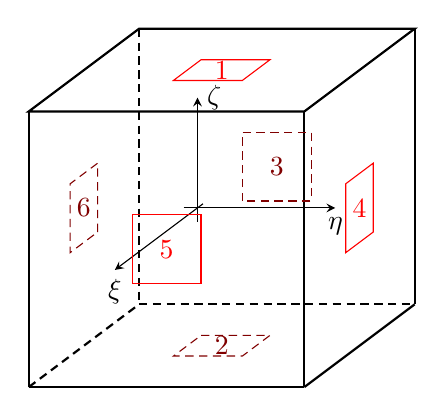
\begin{tikzpicture}[scale=1.75,>=stealth,
  x={(-0.4cm,-0.3cm)}, y={ (1cm,0cm) }, z={(0cm,1cm)}]
 \tikzstyle{background} = [densely dashed]
 \newcommand{\fs}{0.25}
 
% Coord.sys. (shifted for readability)
 \draw[->,xshift=-5] (-0.1,0,0) -- (1.5,0,0) node[at end,below] {$\xi$};
 \draw[->,xshift=-5] (0,-0.1,0) -- (0,1,0) node[at end,below] {$\eta$};
 \draw[->,xshift=-5] (0,0,-0.1) -- (0,0,0.8) node[at end,right] {$\zeta$};

% Can't use rectangle in 3d
 \draw[thick] (-1,-1,1) -- (-1,1,1) -- (1,1,1) -- (1,-1,1) -- cycle;
 \draw[thick,background] (-1,-1,-1) -- (-1,1,-1);
 \draw[thick] (-1,1,-1)-- (1,1,-1);
 \draw[thick] (1,1,-1) -- (1,-1,-1);
 \draw[thick,background] (1,-1,-1) -- (-1,-1,-1);
 \draw[thick,background] (-1,-1,1) -- (-1,-1,-1);
 \draw[thick] (-1,1,1) -- (-1,1,-1);
 \draw[thick] (1,-1,1) -- (1,-1,-1);
 \draw[thick] (1,1,1) -- (1,1,-1);

% Faces
 \draw[red] (1,-\fs,-\fs) -- (1,-\fs,\fs) -- (1,\fs,\fs) -- (1,\fs,-\fs) -- cycle;
 \node[red] at (1,0,0) {5};
 \draw[red] (-\fs,1,-\fs) -- (-\fs,1,\fs) -- (\fs,1,\fs) -- (\fs,1,-\fs) -- cycle;
 \node[red] at (0,1,0) {4};
 \draw[red] (-\fs,-\fs,1) -- (-\fs,\fs,1) -- (\fs,\fs,1) -- (\fs,-\fs,1) -- cycle;
 \node[red] at (0,0,1) {1};
 \draw[red!50!black,background] (-1,-\fs,-\fs) -- (-1,-\fs,\fs) -- (-1,\fs,\fs) -- (-1,\fs,-\fs) -- cycle;
 \node[red!50!black] at (-1,0,0) {3};
 \draw[red!50!black,background] (-\fs,-1,-\fs) -- (-\fs,-1,\fs) -- (\fs,-1,\fs) -- (\fs,-1,-\fs) -- cycle;
 \node[red!50!black] at (0,-1,0) {6};
 \draw[red!50!black,background] (-\fs,-\fs,-1) -- (-\fs,\fs,-1) -- (\fs,\fs,-1) -- (\fs,-\fs,-1) -- cycle;
 \node[red!50!black] at (0,0,-1) {2};

% Edges
% \node[blue,above] at (-1,0,1) {1};
% \node[blue,above left] at (0,1,1) {2};
% \node[blue,above left] at (1,0,1) {3};
% \node[blue,above left] at (0,-1,1) {4};
% \node[blue!50!black,left] at (-1,-1,0) {5};
% \node[blue,left] at (-1,1,0) {6};
% \node[blue,left] at (1,1,0) {7};
% \node[blue,left] at (1,-1,0) {8};
% \node[blue!50!black,above] at (-1,0,-1) {9};
% \node[blue,above left] at (0,1,-1) {10};
% \node[blue,above left] at (1,0,-1) {11};
% \node[blue!50!black,above left] at (0,-1,-1) {12};
\end{tikzpicture}
}
 \end{makeimage}
 \caption{QSpace element.}
\end{figure}

\begin{elementsummary}{qspace}{Quadratic isoparametric brick element}{\optField{NIP}{in}}{qspace element summary}{qspacesummary}
\elementParam{\param{NIP}: allows to set the number of integration points (possible completions are 1, 8 (default), or 27).}
\elementDescription{Unknowns}{Three dofs (u-displacement, v-displacement, w-displacement) are required in each node.}
\elementDescription{Approximation}{Quadratic approximation of displacement and geometry.}
\elementDescription{Integration}{Full integration of all strain components.}
\elementDescription{Features}{-}
\elementDescription{CS properties}{-}
\elementDescription{Loads}{-}
\elementDescription{Nlgeo}{0,1,2.}
\elementDescription{Status}{Reliable}
\end{elementsummary}


\subsubsection{LTRSpace element}
Implementation of tetrahedra four-node finite element. 
Each node has 3 degrees of freedom. The element features are summarized in Table~\ref{LTRSpacesummary}.
Following node numbering convention is adopted (see also Fig.~\ref{lintetrahedron_fig}):
\begin{itemize}
\item Select a face that will contain the first three corners. The excluded corner will be the last one.
\item Number these three corners in a counterclockwise sense when looking at the face from the
      excluded corner.
\end{itemize}
 
\begin{figure}[htb]
 \centering
 \begin{makeimage}
  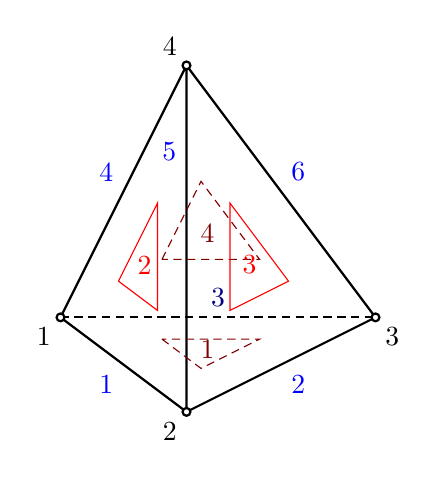
\begin{tikzpicture}[scale=4,>=stealth,x={(1cm,0cm)}, y={ (0.4cm,-0.3cm) }, z={(0.4cm,0.8cm)}]
 \tikzstyle{elemnode} = [draw=black,thick,fill=white,circle,inner sep=1]
 \tikzstyle{background} = [densely dashed]
 \newcommand{\fs}{0.23}
 
% Can't use rectangle in 3d
 \draw[thick,background] (0,0,0) -- (1,0,0) node[midway,above,blue!50!black] {3};
 \draw[thick] (0,0,1) -- (0,0,0) node[midway,above left,blue] {4}
                      -- (0,1,0) node[midway,below left,blue] {1} 
                      -- (1,0,0) node[midway,below right,blue] {2}
                      -- (0,0,1) node[midway,above right,blue] {6}
                      -- (0,1,0) node[near start,left,blue] {5};

% Nodes
 \node[elemnode] (n1) at (0,0,0) {}; \node[below left] at (n1) {1};
 \node[elemnode] (n2) at (0,1,0) {}; \node[below left] at (n2) {2};
 \node[elemnode] (n3) at (1,0,0) {}; \node[below right] at (n3) {3};
 \node[elemnode] (n4) at (0,0,1) {}; \node[above left] at (n4) {4};

% Faces
 \draw[red!50!black,background] (\fs,\fs,0) -- (\fs,1-2*\fs,0) -- (1-2*\fs,\fs,0) -- cycle;
 \node[red!50!black] at (1/3,1/3,0) {1};
 \draw[red!50!black,background] (\fs,0,\fs) -- (\fs,0,1-2*\fs) -- (1-2*\fs,0,\fs) -- cycle;
 \node[red!50!black] at (1/3,0,1/3) {4};

 \draw[red] (0,\fs,\fs) -- (0,\fs,1-2*\fs) -- (0,1-2*\fs,\fs) -- cycle;
 \node[red] at (0,1/3,1/3) {2};
 \draw[red] (1-2*\fs,\fs,\fs) -- (\fs,1-2*\fs,\fs) -- (\fs,\fs,1-2*\fs) -- cycle;
 \node[red] at (1/3,1/3,1/3) {3};


\end{tikzpicture}

 \end{makeimage}
 \caption{LTRSpace element. Definition and node numbering convention.}
 \label{lintetrahedron_fig}
\end{figure}

\begin{elementsummary}{LTRSpace}{Linear tetrahedra element}{-}{LTRSpace element summary}{LTRSpacesummary}
%\elementParam{\param{NIP}: allows to set the number of integration points (possible completions are 1, 8 (default), or 27).}
\elementDescription{Unknowns}{Three dofs (u-displacement, v-displacement, w-displacement) are required in each node.}
\elementDescription{Approximation}{ Linear approximation of displacements and geometry using linear volume coordinates.}
\elementDescription{Integration}{Full integration of all strain components using four point Gauss integration formula.}
\elementDescription{Features}{Adaptivity support, Geometric nonlinearity support.}
\elementDescription{CS properties}{-}
\elementDescription{Loads}{Surface and Edge loadings supported.}
\elementDescription{Nlgeo}{0,1,2.}
\elementDescription{Status}{Reliable}
\end{elementsummary}


\subsubsection{QTRSpace element}
Implementation of tetrahedra ten-node finite element. 
Each node has 3 degrees of freedom. The element features are summarized in Table~\ref{QTRSpacesummary}.
Following node numbering convention is adopted (see also Fig.~\ref{qtetrahedron_fig}):

\begin{figure}[htb]
 \centering
 \begin{makeimage}
  \raisebox{-0.5\height}{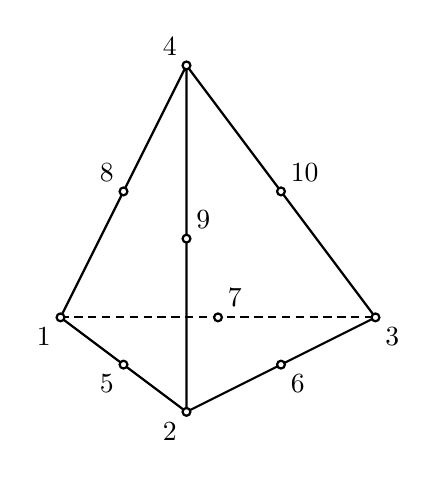
\begin{tikzpicture}[scale=4,>=stealth,x={(1cm,0cm)}, y={ (0.4cm,-0.3cm) }, z={(0.4cm,0.8cm)}]
 \tikzstyle{elemnode} = [draw=black,thick,fill=white,circle,inner sep=1]
 \tikzstyle{background} = [densely dashed]
 \newcommand{\fs}{0.23}
 
% Can't use rectangle in 3d
 \draw[thick,background] (0,0,0) -- (1,0,0) node[midway,above,blue!50!black]{};
 \draw[thick] (0,0,1) -- (0,0,0) node[midway,above left,blue] {}
                      -- (0,1,0) node[midway,below left,blue] {}
                      -- (1,0,0) node[midway,below right,blue]{}
                      -- (0,0,1) node[midway,above right,blue]{}
                      -- (0,1,0) node[near start,left,blue] {};
% Nodes
 \node[elemnode] (n1) at (0,0,0) {}; \node[below left] at (n1) {1};
 \node[elemnode] (n2) at (0,1,0) {}; \node[below left] at (n2) {2};
 \node[elemnode] (n3) at (1,0,0) {}; \node[below right] at (n3) {3};
 \node[elemnode] (n4) at (0,0,1) {}; \node[above left] at (n4) {4};
 \node[elemnode] (n5) at (0,0.5,0) {}; \node[below left] at (n5) {5};
 \node[elemnode] (n6) at (0.5,0.5,0) {}; \node[below right] at (n6) {6};
 \node[elemnode] (n7) at (0.5,0.,0) {}; \node[above right] at (n7) {7};
 \node[elemnode] (n8) at (0,0,0.5) {}; \node[above left] at (n8) {8};
 \node[elemnode] (n9) at (0,0.5,0.5) {}; \node[above right] at (n9) {9};
 \node[elemnode] (n10) at (0.5,0,0.5) {}; \node[above right] at (n10) {10};


\end{tikzpicture}
}
  \raisebox{-0.5\height}{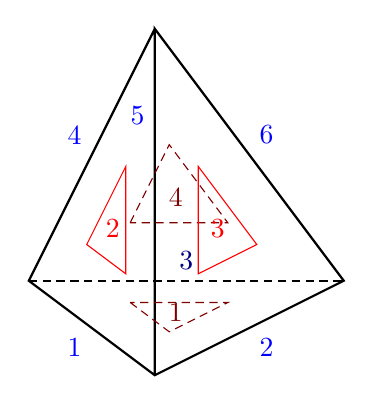
\begin{tikzpicture}[scale=4,>=stealth,x={(1cm,0cm)}, y={ (0.4cm,-0.3cm) }, z={(0.4cm,0.8cm)}]
 \tikzstyle{elemnode} = [fill,circle,inner sep=2]
 \tikzstyle{background} = [densely dashed]
 \newcommand{\fs}{0.23}
 
% Can't use rectangle in 3d
 \draw[thick,background] (0,0,0) -- (1,0,0) node[midway,above,blue!50!black] {3};
 \draw[thick] (0,0,1) -- (0,0,0) node[midway,above left,blue] {4}
                      -- (0,1,0) node[midway,below left,blue] {1} 
                      -- (1,0,0) node[midway,below right,blue] {2}
                      -- (0,0,1) node[midway,above right,blue] {6}
                      -- (0,1,0) node[near start,left,blue] {5};

% Faces
 \draw[red!50!black,background] (\fs,\fs,0) -- (\fs,1-2*\fs,0) -- (1-2*\fs,\fs,0) -- cycle;
 \node[red!50!black] at (1/3,1/3,0) {1};
 \draw[red!50!black,background] (\fs,0,\fs) -- (\fs,0,1-2*\fs) -- (1-2*\fs,0,\fs) -- cycle;
 \node[red!50!black] at (1/3,0,1/3) {4};

 \draw[red] (0,\fs,\fs) -- (0,\fs,1-2*\fs) -- (0,1-2*\fs,\fs) -- cycle;
 \node[red] at (0,1/3,1/3) {2};
 \draw[red] (1-2*\fs,\fs,\fs) -- (\fs,1-2*\fs,\fs) -- (\fs,\fs,1-2*\fs) -- cycle;
 \node[red] at (1/3,1/3,1/3) {3};


\end{tikzpicture}
}
 \end{makeimage}
 \caption{QTRSpace element. Definition and node numbering convention.}
  \label{qtetrahedron_fig}
\end{figure}

\begin{elementsummary}{QTRSpace}{3D tetrahedra element with quadratic interpolation}{\optField{NIP}{in}}{QTRSpace element summary}{QTRSpacesummary}
\elementParam{\param{NIP}: allows to alter  the default integration formula (possible completions are 1, 4 (default), 5, 11, 15, 24, and 45 point intergartion formulas).}
\elementDescription{Unknowns}{Three dofs (u-displacement, v-displacement, w-displacement) are required in each node.}
\elementDescription{Approximation}{Quadratic approximation of displacements and geometry using linear volume coordinates.}
\elementDescription{Integration}{Full integration of all strain components using four point Gauss integration formula.}
\elementDescription{Features}{-}
\elementDescription{CS properties}{-}
\elementDescription{Loads}{-}
\elementDescription{Nlgeo}{0,1,2.}
\elementDescription{Status}{Reliable}
\end{elementsummary}


\subsubsection{LWedge element}
Implementation of wedge six-node finite element. 
Each node has 3 degrees of freedom. The element features are summarized in Table~\ref{LWedgesummary}.
Following node numbering convention is adopted (see also Fig.~\ref{linwedge_fig}):

\begin{figure}[htb]
 \centering
 \begin{makeimage}
  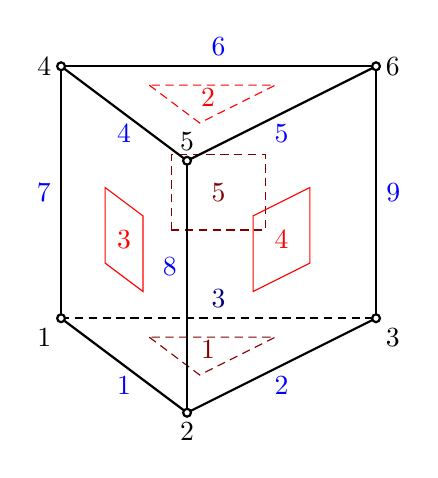
\begin{tikzpicture}[scale=4,>=stealth,x={(1cm,0cm)}, y={ (0.4cm,-0.3cm) }, z={(0.0cm,0.8cm)}]
 %\tikzstyle{elemnode} = [fill,circle,inner sep=2]
 \tikzstyle{elemnode} = [draw=black,thick,fill=white,circle,inner sep=1]
 \tikzstyle{background} = [densely dashed]
 \newcommand{\fs}{0.20}
 \newcommand{\fsb}{0.35}
 
  \coordinate (n1) at (0,0,0);
  \coordinate (n2) at (0,1,0);
  \coordinate (n3) at (1,0,0);
  \coordinate (n4) at (0,0,1);
  \coordinate (n5) at (0,1,1);
  \coordinate (n6) at (1,0,1);

  % Faces behind
  \draw[red!50!black,background] (\fs,\fs,0) -- (\fs,1-2*\fs,0) -- (1-2*\fs,\fs,0) -- cycle;
  \node[red!50!black] at (1/3,1/3,0) {1};
  \draw[red!50!black,background] (\fsb,0,\fsb) -- (\fsb,0,1-\fsb) -- (1-\fsb,0,1-\fsb) -- (1-\fsb,0,\fsb) -- cycle;
  \node[red!50!black] at (1/2,0,1/2) {5};


  % Can't use rectangle in 3d
  \draw[thick,background] (n1) -- (n3) node[midway,above,blue!50!black] {3};
  \draw[thick] (n2) -- (n1) node[midway,below,blue] {1};
  \draw[thick] (n2) -- (n3) node[midway,below,blue] {2};
  \draw[thick] (n5) -- (n4) node[midway,below,blue] {4};
  \draw[thick] (n5) -- (n6) node[midway,below,blue] {5};
  \draw[thick] (n4) -- (n6) node[midway,above,blue] {6};
  \draw[thick] (n1) -- (n4) node[midway,left,blue] {7};
  \draw[thick] (n2) -- (n5) node[midway,above left,blue] {8};
  \draw[thick] (n3) -- (n6) node[midway,right,blue] {9};

  % Nodes
  \node[elemnode] at (n1) {}; \node[below left] at (n1) {1};
  \node[elemnode] at (n2) {}; \node[below] at (n2) {2};
  \node[elemnode] at (n3) {}; \node[below right] at (n3) {3};
  \node[elemnode] at (n4) {}; \node[left] at (n4) {4};
  \node[elemnode] at (n5) {}; \node[above] at (n5) {5};
  \node[elemnode] at (n6) {}; \node[right] at (n6) {6};

  % Faces
  \draw[red,background] (\fs,\fs,1) -- (\fs,1-2*\fs,1) -- (1-2*\fs,\fs,1) -- cycle;
  \node[red] at (1/3,1/3,1) {2};

  \draw[red] (0,\fsb,\fsb) -- (0,\fsb,1-\fsb) -- (0,1-\fsb,1-\fsb) -- (0,1-\fsb,\fsb) -- cycle;
  \node[red] at (0,1/2,1/2) {3};

  \draw[red] (\fsb,1-\fsb,\fsb) -- (1-\fsb,\fsb,\fsb) -- (1-\fsb,\fsb,1-\fsb) -- (\fsb,1-\fsb,1-\fsb) -- cycle;
  \node[red] at (1/2,1/2,1/2) {4};

\end{tikzpicture}

 \end{makeimage}
  \caption{LWedge element. Node numbering convention in black, edge numbering in blue and face numbering in red.}
  \label{linwedge_fig}
\end{figure}

\begin{elementsummary}{LWedge}{3D wedge six-node finite element with linear interpolation}{\optField{NIP}{in}}{LWedge element summary}{LWedgesummary}
\elementParam{\param{NIP}: allows to alter  the default integration formula (possible completions are 2 (default) and 9 point integration formulas).}
\elementDescription{Unknowns}{Three dofs (u-displacement, v-displacement, w-displacement) are required in each node.}
\elementDescription{Approximation}{Linear approximation of displacements and geometry.}
\elementDescription{Integration}{Full integration of all strain components using four point Gauss integration formula.}
\elementDescription{Features}{-}
\elementDescription{CS properties}{-}
\elementDescription{Loads}{-}
\elementDescription{Nlgeo}{0,1,2.}
\elementDescription{Status}{Reliable}
\end{elementsummary}

\subsubsection{QWedge element}
Implementation of wedge fifteen-node finite element. 
Each node has 3 degrees of freedom. The element features are summarized in Table~\ref{QWedgesummary}.
Following node numbering convention is adopted (see also Fig.~\ref{qwedge_fig}):

\begin{figure}[htb]
 \centering
 \begin{makeimage}
  \raisebox{-1.\height}{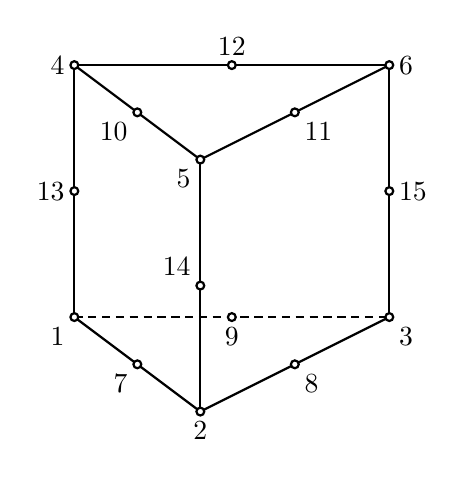
\begin{tikzpicture}[scale=4,>=stealth,x={(1cm,0cm)}, y={ (0.4cm,-0.3cm) }, z={(0.0cm,0.8cm)}]
 \tikzstyle{elemnode} = [draw=black,thick,fill=white,circle,inner sep=1]
 \tikzstyle{background} = [densely dashed]

  \coordinate (n1) at (0,0,0);
  \coordinate (n2) at (0,1,0);
  \coordinate (n3) at (1,0,0);
  \coordinate (n4) at (0,0,1);
  \coordinate (n5) at (0,1,1);
  \coordinate (n6) at (1,0,1);

  % Can't use rectangle in 3d
  \draw[thick,background] (n1) -- (n3) coordinate[midway] (e3);
  \draw[thick] (n2) -- (n1) coordinate[midway] (e1);
  \draw[thick] (n2) -- (n3) coordinate[midway] (e2);
  \draw[thick] (n5) -- (n4) coordinate[midway] (e4);
  \draw[thick] (n5) -- (n6) coordinate[midway] (e5);
  \draw[thick] (n4) -- (n6) coordinate[midway] (e6);
  \draw[thick] (n1) -- (n4) coordinate[midway] (e7);
  \draw[thick] (n2) -- (n5) coordinate[midway] (e8);
  \draw[thick] (n3) -- (n6) coordinate[midway] (e9);

  % Nodes
  \node[elemnode] at (n1) {}; \node[below left ] at (n1) {1};
  \node[elemnode] at (n2) {}; \node[below      ] at (n2) {2};
  \node[elemnode] at (n3) {}; \node[below right] at (n3) {3};
  \node[elemnode] at (n4) {}; \node[      left ] at (n4) {4};
  \node[elemnode] at (n5) {}; \node[below left ] at (n5) {5};
  \node[elemnode] at (n6) {}; \node[      right] at (n6) {6};

  \node[elemnode] at (e1) {}; \node[below left ] at (e1) {7};
  \node[elemnode] at (e2) {}; \node[below right] at (e2) {8};
  \node[elemnode] at (e3) {}; \node[below      ] at (e3) {9};
  \node[elemnode] at (e4) {}; \node[below left ] at (e4) {10};
  \node[elemnode] at (e5) {}; \node[below right] at (e5) {11};
  \node[elemnode] at (e6) {}; \node[above      ] at (e6) {12};
  \node[elemnode] at (e7) {}; \node[      left ] at (e7) {13};
  \node[elemnode] at (e8) {}; \node[above left ] at (e8) {14};
  \node[elemnode] at (e9) {}; \node[      right] at (e9) {15};

\end{tikzpicture}
}
  \raisebox{-1.\height}{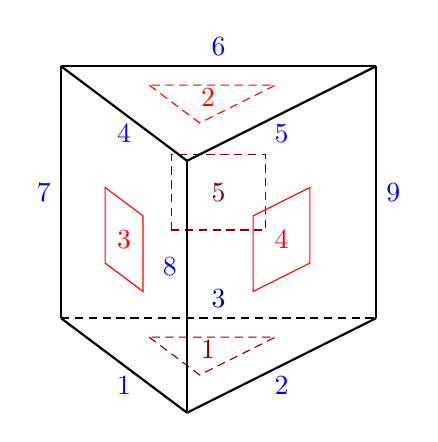
\begin{tikzpicture}[scale=4,>=stealth,x={(1cm,0cm)}, y={ (0.4cm,-0.3cm) }, z={(0.0cm,0.8cm)}]
 %\tikzstyle{elemnode} = [fill,circle,inner sep=2]
 \tikzstyle{elemnode} = [draw=black,thick,fill=white,circle,inner sep=1]
 \tikzstyle{background} = [densely dashed]
 \newcommand{\fs}{0.20}
 \newcommand{\fsb}{0.35}
 
  \coordinate (n1) at (0,0,0);
  \coordinate (n2) at (0,1,0);
  \coordinate (n3) at (1,0,0);
  \coordinate (n4) at (0,0,1);
  \coordinate (n5) at (0,1,1);
  \coordinate (n6) at (1,0,1);

  % Faces behind
  \draw[red!50!black,background] (\fs,\fs,0) -- (\fs,1-2*\fs,0) -- (1-2*\fs,\fs,0) -- cycle;
  \node[red!50!black] at (1/3,1/3,0) {1};
  \draw[red!50!black,background] (\fsb,0,\fsb) -- (\fsb,0,1-\fsb) -- (1-\fsb,0,1-\fsb) -- (1-\fsb,0,\fsb) -- cycle;
  \node[red!50!black] at (1/2,0,1/2) {5};


  % Can't use rectangle in 3d
  \draw[thick,background] (n1) -- (n3) node[midway,above,blue!50!black] {3};
  \draw[thick] (n2) -- (n1) node[midway,below,blue] {1};
  \draw[thick] (n2) -- (n3) node[midway,below,blue] {2};
  \draw[thick] (n5) -- (n4) node[midway,below,blue] {4};
  \draw[thick] (n5) -- (n6) node[midway,below,blue] {5};
  \draw[thick] (n4) -- (n6) node[midway,above,blue] {6};
  \draw[thick] (n1) -- (n4) node[midway,left,blue] {7};
  \draw[thick] (n2) -- (n5) node[midway,above left,blue] {8};
  \draw[thick] (n3) -- (n6) node[midway,right,blue] {9};

  % Faces
  \draw[red,background] (\fs,\fs,1) -- (\fs,1-2*\fs,1) -- (1-2*\fs,\fs,1) -- cycle;
  \node[red] at (1/3,1/3,1) {2};

  \draw[red] (0,\fsb,\fsb) -- (0,\fsb,1-\fsb) -- (0,1-\fsb,1-\fsb) -- (0,1-\fsb,\fsb) -- cycle;
  \node[red] at (0,1/2,1/2) {3};

  \draw[red] (\fsb,1-\fsb,\fsb) -- (1-\fsb,\fsb,\fsb) -- (1-\fsb,\fsb,1-\fsb) -- (\fsb,1-\fsb,1-\fsb) -- cycle;
  \node[red] at (1/2,1/2,1/2) {4};

\end{tikzpicture}
}
 \end{makeimage}
  \caption{QWedge element. Node numbering convention in black, edge numbering in blue and face numbering in red.}
  \label{qwedge_fig}
\end{figure}

\begin{elementsummary}{QWedge}{3D wedge six-node finite element with quadratic interpolation}{\optField{NIP}{in}}{QWedge element summary}{QWedgesummary}
\elementParam{\param{NIP}: allows to alter  the default integration formula (possible completions are 2 (default) and 9 point integration formulas).}
\elementDescription{Unknowns}{Three dofs (u-displacement, v-displacement, w-displacement) are required in each node.}
\elementDescription{Approximation}{Quadratic approximation of displacements and geometry.}
\elementDescription{Integration}{Full integration of all strain components using four point Gauss integration formula.}
\elementDescription{Features}{-}
\elementDescription{CS properties}{-}
\elementDescription{Loads}{-}
\elementDescription{Nlgeo}{0,1,2.}
\elementDescription{Status}{Reliable}
\end{elementsummary}

%-----------------------------------------------------------------------------------------------
\clearpage
\subsection{Interface elements}

Interface elements represent a contact between two adjacent nodes. Interface material specific to interface element needs to be assigned - consult the {\it matlibmanual} for interface support. 

\subsubsection{Interface1d element}
Implementation of one dimensional (slip) interface element. 
This element can connect two separate nodes by specifying the
one-dimensional slip law, that determines the force acting between
these nodes depending on their relative displacement. This element can
be applied in 1D, 2D, and 3D settings (default). The element features are summarized in Table~\ref{Interface1dsummary}.

\begin{elementsummary}{Interface1d}{One dimensional (slip) interface element}{\optField{refnode}{in} \optField{normal}{ra}}{Interface1d element summary}{Interface1dsummary}
\elementParam{\param{refnode}: determines the reference node, which is used to specify a reference direction (the direction vector is obtained by subtracting the coordinates of the first node from the reference node).}
\elementParam{\param{normal}: The reference direction can be directly specified by the optional parameter \param{normal}. Although both \param{refnode} and \param{normal} are optional, at least one of them must be specified.}

\elementDescription{Unknowns}{One, two, or three DOFs (u-displacement, v-displacement,
w-displacement) are required in each node, according to element mode (determined from domain type).}
\elementDescription{Approximation}{-}
\elementDescription{Integration}{-}
\elementDescription{Features}{-}
\elementDescription{CS properties}{-}
\elementDescription{Loads}{-}
\elementDescription{Nlgeo}{0}
\elementDescription{Status}{Reliable}
\elementDescription{Note}{Element requires material model with \_1dInterface support.}
\end{elementsummary}

\subsubsection{Interface2dquad element}
Implementation of a two dimensional interface element with quadratic
approximation of displacement field. Can be used to glue together two elements with quadratic displacement approximation along the shared edge. Note, that the nodes along the interface are doubled, each couple with identical coordinates. Nodes on the negative side are numbered first, followed by nodes on the positive part. Requires material model with \_2dInterface support.  The element features are summarized in Table~\ref{Interface2dquadsummary}.

\begin{figure}[htb]
 \centering
 \begin{makeimage}
 \tikzstyle{elemnode} = [solid,thin,draw,circle,inner sep=1,fill=white]
\begin{tikzpicture}[scale=3,>=stealth]
 \newcommand{\eoff}{0.03}
 \draw[dashed] 
    (0,0) -- (1,0) node[at start,elemnode] {} node[midway,elemnode] {}
    to[out=90,in=-30] node[at start,elemnode] {} node[midway,elemnode] {}
    (0.5,1) -- (0,0) node[at start,elemnode] {} node[midway,elemnode] {};
 
 \draw[dashed,xshift=15,yshift=5] 
    (1,0) to[out=90,in=-30] node[at start,elemnode] {} node[midway,elemnode] {}
    (0.5,1) -- (1.5,1) node[at start,elemnode] {} node[midway,elemnode] {}
    to[out=-90,in=45] node[at start,elemnode] {} node[midway,elemnode] {} (1,0);

 \begin{scope}[xshift=7.5,yshift=2.5]
  \draw[<->] (0.5,1)+(60:0.3) -- (0.5,1) node[at start,left] {$\eta$}
    to[out=-30,in=90] (1,0) -- (1,-0.3) node[at end,right] {$\xi$};

  \draw[thick] (0.5,1)+(60:-\eoff) to[out=-30,in=90] 
    node[at start,elemnode] (n1) {}
    node[at end,elemnode] (n2) {}
    node[midway,elemnode] (n3) {}
    (1-\eoff,0)
    (0.5,1)+(60:\eoff) to[out=-30,in=90] 
    node[at start,elemnode] (n4) {}
    node[at end,elemnode] (n5) {}
    node[midway,elemnode] (n6) {}
    (1+\eoff,0);
   \node[left] at (n1) {1};
   \node[left] at (n2) {2};
   \node[left] at (n3) {3};
   \node[yshift=2,right] at (n4) {4}; % Fine adjustments
   \node[right] at (n5) {5};
   \node[right] at (n6) {6};
 \end{scope}
\end{tikzpicture}
 \end{makeimage}
 \caption{Interface2dquad element with quadratic interpolation. Definition and node numbering convention}
 \label{interf2d_quad_fig}
\end{figure}

\begin{elementsummary}{Interface2dquad}{2D  interface element with quadratic approximation}{-}{Interface2dquad element summary}{Interface2dquadsummary}
%\elementParam{\param{refnode}: determines the reference node, which is used to specify a reference direction (the direction vector is obtained by subtracting the coordinates of the first node from the reference node).}
\elementDescription{Unknowns}{Two dofs (u-displacement, v-displacement) are required in each node.}
\elementDescription{Approximation}{Quadratic approximation of displacements and geometry.}
\elementDescription{Integration}{Full integration of all strain components using four point integration formula.}
\elementDescription{Features}{-}
\elementDescription{CS properties}{-}
\elementDescription{Loads}{-}
\elementDescription{Nlgeo}{0}
\elementDescription{Status}{Reliable}
\elementDescription{Note}{Element requires material model with \_2dInterface support.}
\end{elementsummary}

\subsubsection{Interface3dtrlin element}
Implementation of a three dimensional interface element with linear
approximation of displacement field. Can be used to glue together two elements with linear displacement approximation along the shared triangular surface. Note, that the nodes along the interface are doubled, each couple with identical coordinates. Nodes on the negative surface are numbered first, followed by nodes on the positive part. The numbering of surface nodes on interface determines the positive normal (right hand rule). The surface in the direction of positive normal is the positive surface. Requires material model with \_3dInterface support. The element features are summarized in Table~\ref{Interface3dtrlinsummary}.

\begin{figure}[htb]
 \centering
 \begin{makeimage}
  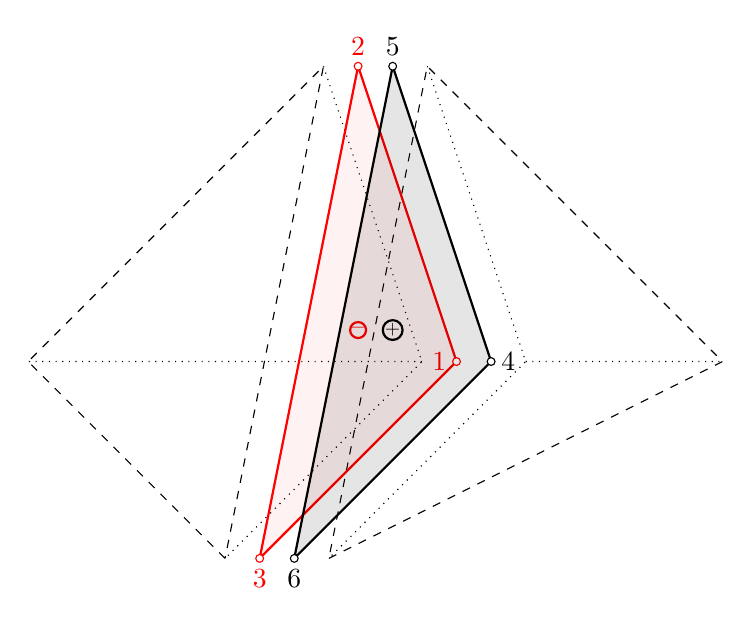
\begin{tikzpicture}[scale=5,>=stealth,
  x={(1cm,0cm)}, y={(-0.5cm,-0.5cm)}, z={(0cm,1cm)}]
 \tikzstyle{elemnode} = [solid,draw,thin,circle,inner sep=1,fill=white]
 
 \begin{scope}
 %\draw[->] (-0.05,0,0) -- (0.5,0,0) node[at end, below] {$x_g$};
 %\draw[->] (0,-0.05,0) -- (0,0.5,0) node[at end, below] {$y_g$};
 %\draw[->] (0,0,-0.05) -- (0,0,0.25) node[at end, right] {$z_g$};
 \end{scope}
 
 \begin{scope}[xshift=-2.5]
  \draw[dotted] (0,0,0) -- (-1,0,0) (0,0.5,1) -- (0,0,0) -- (0,1,0);
  \draw[dashed] (0,1,0) -- (-1,0,0) -- (0,0.5,1) -- cycle;
 \end{scope}

 \begin{scope}[xshift=5]
  \draw[dotted] (0,0,0) -- (0.5,0,0) (0,0.5,1) -- (0,0,0) -- (0,1,0);
  \draw[dashed] (0,1,0) -- (0.5,0,0) -- (0,0.5,1) -- cycle;
 \end{scope}

 \draw[fill=red,opacity=0.05] (0,0,0) -- (0,1,0) -- (0,0.5,1) -- cycle;
 \draw[thick,red] (0,0,0) node[elemnode] {}  node[left] {1}
  -- (0,1,0) node[elemnode] {} node[below] {3}
  -- (0,0.5,1) node[elemnode] {} node[above] {2}
  -- cycle node[draw,circle,inner sep=0] at (0,0.5,0.33) {\scriptsize $-$};

 \draw[fill=black,opacity=0.1,xshift=2.5] (0,0,0) -- (0,1,0) -- (0,0.5,1) -- cycle;
 \draw[thick,xshift=2.5] (0,0,0) node[elemnode] {} node[right] {4}
  -- (0,1,0) node[elemnode] {} node[below] {6}
  -- (0,0.5,1) node[elemnode] {} node[above] {5}
  -- cycle node[draw,circle,inner sep=0] at (0,0.5,0.33) {\scriptsize $+$};

\end{tikzpicture}

 \end{makeimage}
 \caption{Interface3dtrlin element with linear interpolation. Definition and node numbering convention}
 \label{interf3d_lin_fig}
\end{figure}

\begin{elementsummary}{Interface3dtrlin}{3D  interface element with linear approximation}{-}{Interface3dtrlin element summary}{Interface3dtrlinsummary}
%\elementParam{\param{refnode}: determines the reference node, which is used to specify a reference direction (the direction vector is obtained by subtracting the coordinates of the first node from the reference node).}
\elementDescription{Unknowns}{Three dofs (u-displacement, v-displacement, w-displacement) are required in each node.}
\elementDescription{Approximation}{Linear approximation of displacements and geometry.}
\elementDescription{Integration}{Full integration of all components using one point integration formula.}
\elementDescription{Features}{-}
\elementDescription{CS properties}{-}
\elementDescription{Loads}{-}
\elementDescription{Nlgeo}{0}
\elementDescription{Status}{Reliable}
\elementDescription{Note}{Element requires material model with \_3dInterface support.}
\end{elementsummary}

%-----------------------------------------------------------------------------------------------
\clearpage
\subsection{Iso Geometric Analysis based (IGA) elements}
The following record describes the common part of IGA element record:
 
\noindent
\begin{record}
  \recentry{\entKeyword{IGAElement}}{\componentNum}
  \recentry{}{\field{mat}{in} \field{crossSect}{in} \field{nodes}{ia}}
  %% interpolation specific
  \recentry{}{\field{knotvectoru}{ra} \field{knotvectorv}{ra} \field{knotvectorw}{ra}}
  \recentry{}{\optField{knotmultiplicityu}{ia} \optField{knotmultiplicityv}{ia}}
  \recentry{}{\optField{knotmultiplicityw}{ia}}
  \recentry{}{\field{degree}{ia} \field{nip}{ia}}
  %% parallel stuff
  \recentry{}{\PoptField{partitions}{ia} \PoptField{remote}{}}
\end{record}
The \param{knotvectoru}, \param{knotvectorv}, and \param{knotvectorw} parameters specify  knot vectors in individual parametric directions, considering only distinct knots. Open knot vector is always assumed, so the multiplicity of the first and last knot should be equal to $p+1$, where $p$ is polynomial degree in coresponding direction (determined by \param{degree} parameter, see further).\\
The knot multiplicity can be set using optional parameters \param{knotmultiplicityu}, \param{knotmultiplicityv}, and \param{knotmultiplicityw}. By default, the open knot vector is assumed and multiplicity of internal knots is assumed to be equal to one. Note, that total number of knots in particular direction (including multiplicity) must be equal to number of control points in this direction increased by degree in this direction plus 1.\\
The degree of approximation for each parametric direction is determined from \param{degree} array, dimension of which is equal to number of spatial dimensions of the problem.\\
In case of elements with BSpline or Nurbs interpolation, the nodes forming the rectangular array of control points of the element are ordered in a such way, that u-index is changing most quickly, and w-index (or v-index in case of 2d problems) most slowly. In case of elements with T-spline interpolation, the nodes forming the T-mesh of the element are ordered arbitrarily.

The supported \entKeyword{IGAElement} values are following:\\
\elemkeyword{bsplineplanestresselement}\\
\descitem{Parameters} None.\\
\elemkeyword{nurbsplanestresselement}\\
\descitem{Parameters} None.\\
\elemkeyword{nurbs3delement}\\
\descitem{Parameters} None.\\
\elemkeyword{tsplineplanestresselement}\\
\descitem{Parameters} \field{localindexknotvectoru}{in} \field{localindexknotvectorv}{in} \field{localindexknotvectorw}{in}\\
The parameters \param{localindexknotvectoru}, \param{localindexknotvectorv},\\ and \param{localindexknotvectorw} defined by the indices to global knot vectors (given by \param{knotvectoru}, \param{knotvectorv}, and \param{knotvectorw} parameters) specify the local knot vectors for each control point of T-mesh (node) in the same order as the nodes have been specified for the element. The local knot vector in a particular direction has $p+2$ entries, where the $p$ is the polynomial degree in that direction.


%-----------------------------------------------------------------------------------------------
\clearpage
\subsection{Special elements}
\subsubsection{LumpedMass element}
This element, defined by a single node, allows to introduce additional concentrated mass and/or rotational inertias in a node.
A different mass and rotary inertia may be assigned to each coordinate direction. At present, individual mass/inertia components can be specified for  every degree of freedom of element node. Only displacement and rotational degrees od freedom are considered.  The element features are summarized in Table~\ref{LumpedMasssummary}.

\begin{elementsummary}{LumpedMass}{Lumped mass element}{\field{components}{ra}}{LumpedMass element summary}{LumpedMasssummary}
\elementParam{\param{components}: allows to specify additional concentrated mass components (Force*Time$^2$/Length) and rotary inertias (Force*Length*Time$^2$) about the nodal coordinate axes. Only displacement and rotational degrees of freedom are considered. The individual DOFs are ordered according to following rule: first, displacement degrees of freedom in the direction of x,y, and z axes (if any), followed by rotational DOFs around x,y, and z axes (if any).}
\elementDescription{Unknowns}{Only displacement and roational DOFs are considered ($D_u$, $D_v$, $D_w$, $R_u$, $R_v$, and $R_w$).}
\elementDescription{Approximation}{-}
\elementDescription{Integration}{-}
\elementDescription{Features}{-}
\elementDescription{CS properties}{-}
\elementDescription{Loads}{-}
\elementDescription{Status}{Reliable}
\end{elementsummary}

\subsubsection{Spring element}
This element represent longitudial or torsional spring element. It is defined by two nodes, orientation and a spring constant.
The spring element has no mass associated, the mass can be added using LumpedMass element. The spring is linear and works the same way in tension or in compression. The element features are summarized in Table~\ref{Springsummary}.

\begin{elementsummary}{Spring}{Spring element}{\field{mode}{in} \field{k}{rn} \field{orientation}{ra}}{Spring element summary}{Springsummary}
\elementParam{\param{mode}: defines the type of spring element (see Table~\ref{spring_mode_table}).}
\elementParam{\param{k}:  determines the spring constant, corresponding units are [Force/Length] for longitudinal spring and [Force*Length/Radian] for torsional spring.}
\elementParam{\param{orientation}:defines orientation vector of spring element (of size 3) - for longitudinal spring it defines the direction of spring, for torsional spring it defines the axis of rotation.}
\elementDescription{Note}{the spring element nodes doesn't need to be coincident, but the spring orientation is always determined by \param{orientation} vector.}
\end{elementsummary}

\begin{table}
  \centering
  \begin{tabular}{lll}
    \hline
    mode & description\\
    \hline
    0 & 1D spring element along x-axis,\\
    & requires D\_u DOF in each node, orientation vector is \{1,0,0\}\\
    1 & 2D spring element in xy plane,\\
    & requires D\_u and D\_v DOFs in each node \\
    & (orientation vector should be in xy plane)\\
    2 & 2D torsional spring element in xz plane,\\
    & requires R\_v DOFs in each node\\
    3 & 3D spring element in space,\\
    & requires D\_u, D\_v, and D\_w DOFs in each node\\
    4 & 3D torsional spring in space,\\
    & requires R\_u, R\_v, and R\_w DOFs in each node\\
    \hline
  \end{tabular}
  \caption{Supported spring element modes } \label{spring_mode_table}
\end{table}

%-----------------------------------------------------------------------------------------------
\clearpage
\subsection{Geometric nonlinear analysis}
To take geometric nonlinearity into account on an element, keyword \param{nlgeo} has to be specified. The \param{nlgeo} parameter defines which type of the strain tensor is computed (see Table~\ref{strain_tensor_table}).
\begin{table}
  \centering
  \begin{tabular}{lll}
    \hline
    nlgeo & strain tensor\\
    \hline
    0 (default) & Small-strain tensor\\
    1 & Green-Lagrange strain tensor\\
    2 & Deformation gradient\\
    \hline
  \end{tabular}
  \caption{Nonlinear geometry modes} \label{strain_tensor_table}
\end{table}

%-----------------------------------------------------------------------------------------------
\clearpage
\section{Elements for Transport problems (TM Module)}
\subsection{2D Elements}
\subsubsection{Quad1ht element}
\label{Quad1ht}
Represents isoparametric four-node quadrilateral finite element for
heat transfer problems. Each node has 1 degree of freedom.
Problem should be defined in x,y plane. The cross section thickness
property is requested form cross section model.
The nodes should be numbered anti-clockwise (positive rotation around
z-axis).  The element features are summarized in Table~\ref{Quad1htsummary}.

\begin{figure}[htb]
 \centering
 \begin{makeimage}
  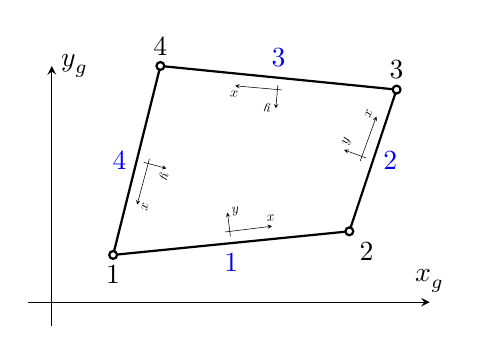
\begin{tikzpicture}[scale=6,>=stealth]
 \tikzstyle{elemnode} = [draw,circle,inner sep=1,fill=white]
 \newcommand{\lcoordsys}[2]{
   \begin{scope}[transform canvas={shift={#2},scale=0.5,rotate=#1}]
    \draw[->] (0,0.05) ++(-0.02,0) -- ++(0.2,0) node[above] {$x$};
    \draw[->] (0,0.05) ++(0,-0.02) -- ++(0,0.1) node[right] {$y$};
   \end{scope}
 }

 \draw[->] (-0.05,0) -- (0.8,0) node[above] {$x_g$};
 \draw[->] (0,-0.05) -- (0,0.5) node[right] {$y_g$};
 
 \draw[thick,xshift=-2] 
     (0.2,0.1)
  -- (0.7,0.15) coordinate[midway] (e1) node[below,midway,blue] {1} node[elemnode] {} node[below right] {2}
  -- (0.8,0.45) coordinate[midway] (e2) node[right,midway,blue] {2} node[elemnode] {} node[above] {3}
  -- (0.3,0.5)  coordinate[midway] (e3) node[above,midway,blue] {3} node[elemnode] {} node[above] {4}
  -- (0.2,0.1)  coordinate[midway] (e4) node[left,midway,blue] {4} node[elemnode] {} node[below] {1};

 \lcoordsys{  7}{(e1)};
 \lcoordsys{ 70}{(e2)};
 \lcoordsys{175}{(e3)};
 \lcoordsys{255}{(e4)};
\end{tikzpicture}

 \end{makeimage}

 \caption{Quad1ht element. Node numbering, Side numbering and
 definition of local edge c.s.(a).}
 \label{Quad1htfig}
\end{figure}

\begin{elementsummary}{Quad1ht}{Isoparametric four-node quadrilateral linear interpolation element for
heat transfer problems}{\optField{NIP}{in}}{Quad1ht element summary}{Quad1htsummary}
\elementParam{\param{NIP}: allows to change the default number of integration point used.}
\elementDescription{Unknowns}{Single dof (T\_f - temperature) is required in each node.}
\elementDescription{Approximation}{Linear approximation of temperature.}
\elementDescription{Integration}{Integration using gauss integration formula
in 4 (the default), 9, or 16 integration points. The default number of
integration point used can be overloaded using \param{NIP} parameter.}
\elementDescription{Loads}{ Body loads are supported. Boundary loads are
supported and computed using numerical integration. The side numbering is
following. Each i-th element side begins in i-th element node and
ends on next element node (i+1-th node or 1-st node, in the case of 
side number 4). The local positive edge x-axis coincides with side
direction, the positive local edge y-axis is rotated 90 degrees
anti-clockwise (see fig. (\ref{Quad1htfig})).}
\elementDescription{Features}{-}
\elementDescription{CS properties}{-}
\elementDescription{Status}{}
\end{elementsummary}

\subsubsection{Quad1hmt element}
Represents isoparametric four-node quadrilateral finite element for
heat and mass (one constituent) transfer problems. 
Two dofs (T\_f - temperature and C\_1 - concentration) are required in
each node. Linear approximation of temperature and mass concentration.
Other features are similar to Quad1 element, see section \ref{Quad1ht}.

\subsubsection{Tr1ht element}
\label{Tr1ht}
Implements the linear triangular finite element for heat transfer problems. Each node has 1 degree of freedom.
The cross section thickness property is requested form cross section model.
The node numbering is anti-clockwise. The element features are summarized in Table~\ref{Tr1htsummary}.

\begin{figure}[htb]
 \centering
 \begin{makeimage}
  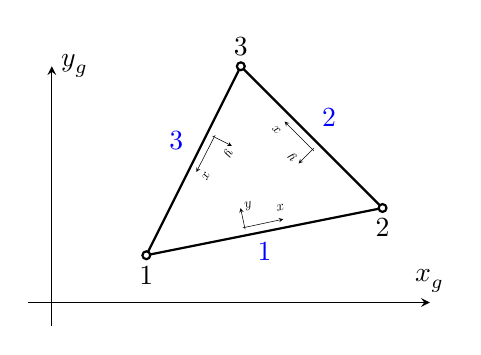
\begin{tikzpicture}[scale=6,>=stealth]
 \tikzstyle{elemnode} = [draw,circle,inner sep=1,fill=white]
 \newcommand{\lcoordsys}[1]{\draw[->] (-0.05,0) -- (1,0) node[above] {$x_{#1}$}; \draw[->] (0,-0.05) -- (0,0.5) node[right] {$y_{#1}$};}
 \draw[->] (-0.05,0) -- (0.8,0) node[above] {$x_g$};
 \draw[->] (0,-0.05) -- (0,0.5) node[right] {$y_g$};
 
 \draw[thick] 
     (0.2,0.1) node[elemnode] {} node[below] {1}
  -- (0.7,0.2) node[elemnode] {} node[below] {2} node[blue,midway,below] {1} coordinate[midway] (e1)
  -- (0.4,0.5) node[elemnode] {} node[above] {3} node[blue,midway,above right] {2} coordinate[midway] (e2)
  -- (0.2,0.1) node[blue,midway,above left] {3} coordinate[midway] (e3);

 \node[yshift=8] at (e1) {\rotatebox{12}{\scalebox{0.5}{\tikz{\lcoordsys{}}}}};
 \node[xshift=-9,yshift=-2] at (e2) {\rotatebox{135}{\scalebox{0.5}{\tikz{\lcoordsys{}}}}};
 \node[xshift=8,yshift=-1] at (e3) {\rotatebox{243}{\scalebox{0.5}{\tikz{\lcoordsys{}}}}};
\end{tikzpicture}

 \end{makeimage}
 \caption{Tr1ht element - node and side numbering.}
 \label{Tr1htfig}
\end{figure}

\begin{elementsummary}{Tr1ht}{triangular finite element with linear approximation for heat transfer problems}{-}{Tr1ht element summary}{Tr1htsummary}
%\elementParam{\param{NIP}: allows to change the default number of integration point used.}
\elementDescription{Unknowns}{Single dof (T\_f - temperature) is required in each node.}
\elementDescription{Approximation}{Linear approximation of temperature.}
\elementDescription{Integration}{Integration using one point gauss integration formula.}
\elementDescription{Loads}{Body loads are supported. Boundary loads are
supported and are computed  using numerical integration. The side numbering is
following. Each i-th element side begins in i-th element node and
ends on next element node (i+1-th node or 1-st node, in the case of 
side number 3). The local positive edge x-axis coincides with side
direction, the positive local edge y-axis is rotated 90 degrees
anti-clockwise (see fig. (\ref{Tr1htfig})).}
\elementDescription{Features}{-}
\elementDescription{CS properties}{-}
\elementDescription{Status}{}
\end{elementsummary}

%-----------------------------------------------------------------------------------------------
\clearpage
\subsection{Axisymmetric Elements}
\subsubsection{Quadaxisym1ht element}
Isoparametric four-node quadrilateral finite element for
axisymmetric heat transfer problems. The element description is
similar to Quad1 element, see section \ref{Quad1ht}.


\subsubsection{Traxisym1ht element}
Linear triangular finite element for axisymmetric heat transfer
problems. The element description is
similar to Tr1ht element, see section \ref{Tr1ht}.

%-----------------------------------------------------------------------------------------------
\clearpage
\subsection{3D Elements}
\subsubsection{Tetrah1ht - tetrahedral 3D element}
Represents isoparametric four-node tetrahedral element. Each node has 1 degree of freedom.
The same numbering convection is adopted as in mechanics, see Fig.~\ref{lintetrahedron_fig}. The element features are summarized in Table~\ref{Tetrah1htsummary}.

\begin{elementsummary}{Tetrah1ht}{Isoparametric, four-node tetrahedral element with linear approximation for heat transfer problems}{\optField{NIP}{in}}{Tetrah1ht element summary}{Tetrah1htsummary}
\elementParam{\param{NIP}: allows to change the default number of integration point used.}
\elementDescription{Unknowns}{Single dof (T\_f - temperature) is required in each node.}
\elementDescription{Approximation}{Linear approximation of temperature.}
\elementDescription{Integration}{Integration using gauss integration formula
in 1 (the default), or 4 integration points. The default number of
integration point used can be overloaded using \param{NIP} parameter.}
\elementDescription{Loads}{Body loads are supported. Boundary loads are
supported and computed using numerical integration. The side and
surface numbering is shown in Fig.~\ref{lintetrahedron_fig}.}
\elementDescription{Features}{-}
\elementDescription{CS properties}{-}
\elementDescription{Status}{}
\end{elementsummary}


\subsubsection{Brick1ht - hexahedral 3D element}
\label{Brick1ht}
Represents isoparametric eight-node brick/hexahedron finite element for
heat transfer problems. Each node has 1 degree of freedom. The element features are summarized in Table~\ref{Brick1htsummary}.

\begin{figure}[htb]
 \centering
 \begin{makeimage}
  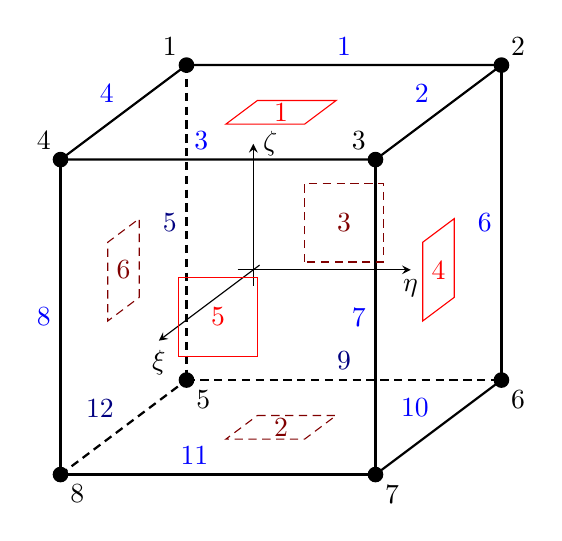
\begin{tikzpicture}[scale=2,>=stealth,
  x={(-0.4cm,-0.3cm)}, y={ (1cm,0cm) }, z={(0cm,1cm)}]
 \tikzstyle{elemnode} = [fill,circle,inner sep=2]
 \tikzstyle{background} = [densely dashed]
 \newcommand{\fs}{0.25}
 
% Coord.sys. (shifted for readability)
 \draw[->,xshift=-5] (-0.1,0,0) -- (1.5,0,0) node[at end,below] {$\xi$};
 \draw[->,xshift=-5] (0,-0.1,0) -- (0,1,0) node[at end,below] {$\eta$};
 \draw[->,xshift=-5] (0,0,-0.1) -- (0,0,0.8) node[at end,right] {$\zeta$};

% Can't use rectangle in 3d
 \draw[thick] (-1,-1,1) -- (-1,1,1) -- (1,1,1) -- (1,-1,1) -- cycle;
 \draw[thick,background] (-1,-1,-1) -- (-1,1,-1);
 \draw[thick] (-1,1,-1)-- (1,1,-1);
 \draw[thick] (1,1,-1) -- (1,-1,-1);
 \draw[thick,background] (1,-1,-1) -- (-1,-1,-1);
 \draw[thick,background] (-1,-1,1) -- (-1,-1,-1);
 \draw[thick] (-1,1,1) -- (-1,1,-1);
 \draw[thick] (1,-1,1) -- (1,-1,-1);
 \draw[thick] (1,1,1) -- (1,1,-1);

% Faces
 \draw[red] (1,-\fs,-\fs) -- (1,-\fs,\fs) -- (1,\fs,\fs) -- (1,\fs,-\fs) -- cycle;
 \node[red] at (1,0,0) {5};
 \draw[red] (-\fs,1,-\fs) -- (-\fs,1,\fs) -- (\fs,1,\fs) -- (\fs,1,-\fs) -- cycle;
 \node[red] at (0,1,0) {4};
 \draw[red] (-\fs,-\fs,1) -- (-\fs,\fs,1) -- (\fs,\fs,1) -- (\fs,-\fs,1) -- cycle;
 \node[red] at (0,0,1) {1};
 \draw[red!50!black,background] (-1,-\fs,-\fs) -- (-1,-\fs,\fs) -- (-1,\fs,\fs) -- (-1,\fs,-\fs) -- cycle;
 \node[red!50!black] at (-1,0,0) {3};
 \draw[red!50!black,background] (-\fs,-1,-\fs) -- (-\fs,-1,\fs) -- (\fs,-1,\fs) -- (\fs,-1,-\fs) -- cycle;
 \node[red!50!black] at (0,-1,0) {6};
 \draw[red!50!black,background] (-\fs,-\fs,-1) -- (-\fs,\fs,-1) -- (\fs,\fs,-1) -- (\fs,-\fs,-1) -- cycle;
 \node[red!50!black] at (0,0,-1) {2};

% Nodes
 \node[elemnode] (n1) at (-1,-1, 1) {}; \node[above left] at (n1) {1};
 \node[elemnode] (n2) at (-1, 1, 1) {}; \node[above right] at (n2) {2};
 \node[elemnode] (n3) at ( 1, 1, 1) {}; \node[above left] at (n3) {3};
 \node[elemnode] (n4) at ( 1,-1, 1) {}; \node[above left] at (n4) {4};
 \node[elemnode] (n5) at (-1,-1,-1) {}; \node[below right] at (n5) {5};
 \node[elemnode] (n6) at (-1, 1,-1) {}; \node[below right] at (n6) {6};
 \node[elemnode] (n7) at ( 1, 1,-1) {}; \node[below right] at (n7) {7};
 \node[elemnode] (n8) at ( 1,-1,-1) {}; \node[below right] at (n8) {8};

% Edges
 \node[blue,above] at (-1,0,1) {1};
 \node[blue,above left] at (0,1,1) {2};
 \node[blue,above left] at (1,0,1) {3};
 \node[blue,above left] at (0,-1,1) {4};

 \node[blue!50!black,left] at (-1,-1,0) {5};
 \node[blue,left] at (-1,1,0) {6};
 \node[blue,left] at (1,1,0) {7};
 \node[blue,left] at (1,-1,0) {8};

 \node[blue!50!black,above] at (-1,0,-1) {9};
 \node[blue,above left] at (0,1,-1) {10};
 \node[blue,above left] at (1,0,-1) {11};
 \node[blue!50!black,above left] at (0,-1,-1) {12};
\end{tikzpicture}

 \end{makeimage}
 \caption{Brick1ht element. Node numbers are in black, side numbers are in blue,
 and surface numbers are in red.}
 \label{Brick1htfig}
\end{figure}

\begin{elementsummary}{Brick1ht}{Isoparametric, hexahedral 3D element with linear approximation for heat transfer problems}{\optField{NIP}{in}}{Brick1ht element summary}{Brick1htsummary}
\elementParam{\param{NIP}: allows to change the default number of integration point used.}
\elementDescription{Unknowns}{Single dof (T\_f - temperature) is required in each node.}
\elementDescription{Approximation}{Linear approximation of temperature.}
\elementDescription{Integration}{Integration using gauss integration formula
in 8 (the default), or 27 integration points. The default number of
integration point used can be overloaded using \param{NIP} parameter.}
\elementDescription{Loads}{Body loads are supported. Boundary loads are
supported and computed using numerical integration. The side and
surface numbering is shown in fig. (\ref{Brick1htfig})).}
\elementDescription{Features}{-}
\elementDescription{CS properties}{-}
\elementDescription{Status}{}
\end{elementsummary}

\subsubsection{Brick1hmt - hexahedral 3D element}
Represents isoparametric eight-node quadrilateral finite element for
heat and mass (one constituent) transfer problems. 
Two dofs (T\_f - temperature and C\_1 - concentration) are required in
each node. Linear approximation of temperature and mass concentration.
Other features are similar to Brick1 element, see section \ref{Brick1ht}.
%\subsection{Other Elements}

\subsubsection{QBrick1ht - quadratic hexahedral 3D element}\label{QBrick1ht_element}
Implementation of quadratic 3d 20-node 
finite element. Each node has 1 degree of freedom. See section ~\ref{QSpace_element} 
for node numbering order and order of faces. The element features are summarized in Table~\ref{QBrick1htsummary}.

\begin{elementsummary}{QBrick1ht}{Isoparametric, hexahedral 3D element with quadratic approximation for heat transfer problems}{\optField{NIP}{in}}{QBrick1ht element summary}{QBrick1htsummary}
\elementParam{\param{NIP}: allows to change the default number of integration point used, possible values are 8, 27 (default) and 64.}
\elementDescription{Unknowns}{Single dof (T\_f - temperature) is required in each node.}
\elementDescription{Approximation}{Quadratic approximation of temperature and
geometry..}
\elementDescription{Integration}{Integration using gauss integration formula
in 8, 27 (default), or 64 integration points. The default number of
integration point used can be overloaded using \param{NIP} parameter.}
\elementDescription{Loads}{-}
\elementDescription{Features}{-}
\elementDescription{CS properties}{-}
\elementDescription{Status}{}
\end{elementsummary}

\subsubsection{QBrick1hmt - quadratic hexahedral 3D element}
The same element as QBrick1ht for
heat and mass (one constituent) transfer problems. 
Two dofs (T\_f - temperature and C\_1 - concentration) are required in
each node. Linear approximation of temperature and mass concentration.
Other features are similar to QBrick1ht element, see section \ref{QBrick1ht_element}.


%-----------------------------------------------------------------------------------------------
\clearpage
\section{Elements for Fluid Dynamics problems (FM Module)}
\subsection{Stokes' Flow Elements}
Stokes' flow elements neglect acceleration, and thus requires no additional stabilization.

\subsubsection{Tr21Stokes element}
Standard 6 node triangular element for stokes flow, with quadratic geometry, velocity and linear pressure.
Both compressible and incompressible material behavior is supported (and also the seamless transition between the two).
The element features are summarized in Table~\ref{Tr121Stokessummary}.

\begin{elementsummary}{Tr121Stokes}{Standard 6 node triangular element for stokes flow, with quadratic geometry, velocity and linear pressure}{-}{Tr121Stokes element summary}{Tr121Stokessummary}
%\elementParam{\param{NIP}: allows to change the default number of integration point used, possible values are 8, 27 (default) and 64.}
\elementDescription{Unknowns}{Unknown pressure in nodes 1--3 with unknown velocity (V\_u and V\_v) in all 6 nodes.}
\elementDescription{Approximation}{Quadratic approximation of geometry and velocity, linear pressure approximation.}
\elementDescription{Integration}{}
\elementDescription{Features}{-}
\elementDescription{Status}{Reliable}
\end{elementsummary}

\subsubsection{Tet21Stokes element}
Standard 10 node tetrahedral element for stokes flow, with quadratic geometry, velocity and linear pressure. The element features are summarized in Table~\ref{Tet21Stokessummary}.

\begin{elementsummary}{Tet21Stokes}{Standard 10 node tetrahedral element for stokes flow, with quadratic geometry, velocity and linear pressure}{-}{Tet21Stokes element summary}{Tet21Stokessummary}
%\elementParam{\param{NIP}: allows to change the default number of integration point used, possible values are 8, 27 (default) and 64.}
\elementDescription{Unknowns}{Unknown pressure (P\_f) in nodes 1--4, and unknown velocity (V\_u, V\_v, V\_w) in all nodes.}
\elementDescription{Approximation}{Quadratic approximation of geometry and velocity, linear pressure approximation.}
\elementDescription{Integration}{}
\elementDescription{Features}{-}
\elementDescription{Status}{Untested}
\end{elementsummary}

\subsubsection{Hexa21Stokes element}
Standard 27 node hexahedral element for stokes flow, with quadratic geometry, velocity and linear pressure. The element features are summarized in Table~\ref{Hexa21Stokessummary}.

\begin{figure}[htb]
 \centering
 \begin{makeimage}
  \raisebox{-0.5\height}{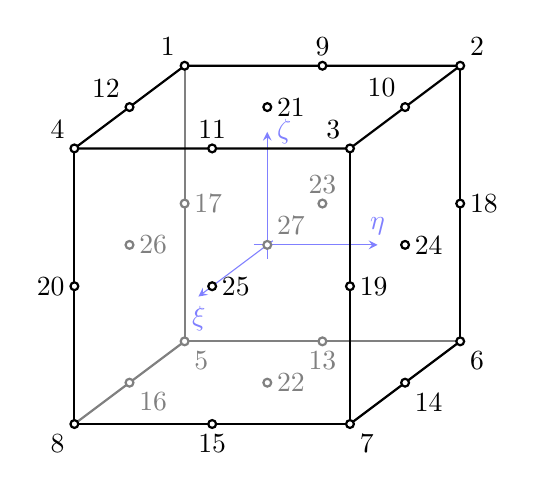
\begin{tikzpicture}[scale=1.75,>=stealth,
  x={(-0.4cm,-0.3cm)}, y={ (1cm,0cm) }, z={(0cm,1cm)}]
 \tikzstyle{elemnode} = [draw=black,thick,fill=white,circle,inner sep=1]
 \tikzstyle{background} = [draw=black!50]
 \tikzstyle{background2} = [black!50]
 
% Coord.sys. (shifted for readability)
 \draw[->,thin,color=blue!50] (-0.1,0,0) -- (1.25,0,0) node[at end,below] {$\xi$};
 \draw[->,thin,color=blue!50] (0,-0.1,0) -- (0,0.8,0) node[at end,above] {$\eta$};
 \draw[->,thin,color=blue!50] (0,0,-0.1) -- (0,0,0.82) node[at end,right] {$\zeta$};

% Can't use rectangle in 3d
 \draw[thick,background] (-1,-1,-1) -- (-1,1,-1);
 \draw[thick,background] (1,-1,-1) -- (-1,-1,-1);
 \draw[thick,background] (-1,-1,1) -- (-1,-1,-1);
 \draw[thick] (-1,-1,1) -- (-1,1,1) -- (1,1,1) -- (1,-1,1) -- cycle;
 \draw[thick] (-1,1,-1)-- (1,1,-1);
 \draw[thick] (1,1,-1) -- (1,-1,-1);
 \draw[thick] (-1,1,1) -- (-1,1,-1);
 \draw[thick] (1,-1,1) -- (1,-1,-1);
 \draw[thick] (1,1,1) -- (1,1,-1);

% Nodes
 \node[elemnode] (n1) at (-1,-1, 1) {}; \node[above left] at (n1) {1};
 \node[elemnode] (n2) at (-1, 1, 1) {}; \node[above right] at (n2) {2};
 \node[elemnode] (n3) at ( 1, 1, 1) {}; \node[above left] at (n3) {3};
 \node[elemnode] (n4) at ( 1,-1, 1) {}; \node[above left] at (n4) {4};
 \node[elemnode,background] (n5) at (-1,-1,-1) {}; \node[below right,background2] at (n5) {5};
 \node[elemnode] (n6) at (-1, 1,-1) {}; \node[below right] at (n6) {6};
 \node[elemnode] (n7) at ( 1, 1,-1) {}; \node[below right] at (n7) {7};
 \node[elemnode] (n8) at ( 1,-1,-1) {}; \node[below left] at (n8) {8};

 \node[elemnode] (n9)  at (-1, 0, 1) {}; \node[above] at (n9) {9};
 \node[elemnode] (n10) at ( 0, 1, 1) {}; \node[above left] at (n10) {10};
 \node[elemnode] (n11) at ( 1, 0, 1) {}; \node[above] at (n11) {11};
 \node[elemnode] (n12) at ( 0,-1, 1) {}; \node[above left] at (n12) {12};

 \node[elemnode,background] (n13) at (-1, 0,-1) {}; \node[below,background2] at (n13) {13};
 \node[elemnode] (n14) at ( 0, 1,-1) {}; \node[below right] at (n14) {14};
 \node[elemnode] (n15) at ( 1, 0,-1) {}; \node[below] at (n15) {15};
 \node[elemnode,background] (n16) at ( 0,-1,-1) {}; \node[below right,background2] at (n16) {16};

 \node[elemnode,background] (n17) at (-1,-1, 0) {}; \node[right,background2] at (n17) {17};
 \node[elemnode] (n18) at (-1, 1, 0) {}; \node[right] at (n18) {18};
 \node[elemnode] (n19) at ( 1, 1, 0) {}; \node[right] at (n19) {19};
 \node[elemnode] (n20) at ( 1,-1, 0) {}; \node[left] at (n20) {20};

 \node[elemnode] (n21) at ( 0, 0, 1) {}; \node[right] at (n21) {21};
 \node[elemnode,background] (n22) at ( 0, 0,-1) {}; \node[right,background2] at (n22) {22};
 \node[elemnode,background] (n23) at (-1, 0, 0) {}; \node[above,background2] at (n23) {23};
 \node[elemnode] (n24) at ( 0, 1, 0) {}; \node[right] at (n24) {24};
 \node[elemnode] (n25) at ( 1, 0, 0) {}; \node[right] at (n25) {25};
 \node[elemnode,background] (n26) at ( 0,-1, 0) {}; \node[right,background2] at (n26) {26};

 \node[elemnode,background] (n27) at ( 0,0, 0) {}; \node[above right,background2] at (n27) {27};

\end{tikzpicture}
}
  \raisebox{-0.5\height}{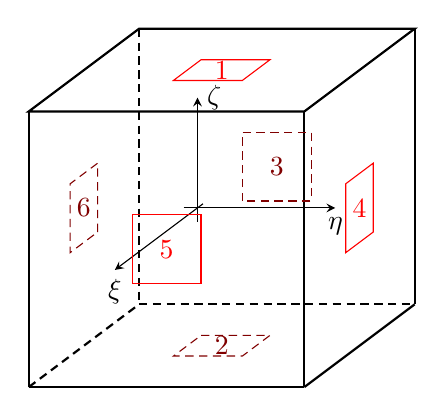
\begin{tikzpicture}[scale=1.75,>=stealth,
  x={(-0.4cm,-0.3cm)}, y={ (1cm,0cm) }, z={(0cm,1cm)}]
 \tikzstyle{background} = [densely dashed]
 \newcommand{\fs}{0.25}
 
% Coord.sys. (shifted for readability)
 \draw[->,xshift=-5] (-0.1,0,0) -- (1.5,0,0) node[at end,below] {$\xi$};
 \draw[->,xshift=-5] (0,-0.1,0) -- (0,1,0) node[at end,below] {$\eta$};
 \draw[->,xshift=-5] (0,0,-0.1) -- (0,0,0.8) node[at end,right] {$\zeta$};

% Can't use rectangle in 3d
 \draw[thick] (-1,-1,1) -- (-1,1,1) -- (1,1,1) -- (1,-1,1) -- cycle;
 \draw[thick,background] (-1,-1,-1) -- (-1,1,-1);
 \draw[thick] (-1,1,-1)-- (1,1,-1);
 \draw[thick] (1,1,-1) -- (1,-1,-1);
 \draw[thick,background] (1,-1,-1) -- (-1,-1,-1);
 \draw[thick,background] (-1,-1,1) -- (-1,-1,-1);
 \draw[thick] (-1,1,1) -- (-1,1,-1);
 \draw[thick] (1,-1,1) -- (1,-1,-1);
 \draw[thick] (1,1,1) -- (1,1,-1);

% Faces
 \draw[red] (1,-\fs,-\fs) -- (1,-\fs,\fs) -- (1,\fs,\fs) -- (1,\fs,-\fs) -- cycle;
 \node[red] at (1,0,0) {5};
 \draw[red] (-\fs,1,-\fs) -- (-\fs,1,\fs) -- (\fs,1,\fs) -- (\fs,1,-\fs) -- cycle;
 \node[red] at (0,1,0) {4};
 \draw[red] (-\fs,-\fs,1) -- (-\fs,\fs,1) -- (\fs,\fs,1) -- (\fs,-\fs,1) -- cycle;
 \node[red] at (0,0,1) {1};
 \draw[red!50!black,background] (-1,-\fs,-\fs) -- (-1,-\fs,\fs) -- (-1,\fs,\fs) -- (-1,\fs,-\fs) -- cycle;
 \node[red!50!black] at (-1,0,0) {3};
 \draw[red!50!black,background] (-\fs,-1,-\fs) -- (-\fs,-1,\fs) -- (\fs,-1,\fs) -- (\fs,-1,-\fs) -- cycle;
 \node[red!50!black] at (0,-1,0) {6};
 \draw[red!50!black,background] (-\fs,-\fs,-1) -- (-\fs,\fs,-1) -- (\fs,\fs,-1) -- (\fs,-\fs,-1) -- cycle;
 \node[red!50!black] at (0,0,-1) {2};

% Edges
% \node[blue,above] at (-1,0,1) {1};
% \node[blue,above left] at (0,1,1) {2};
% \node[blue,above left] at (1,0,1) {3};
% \node[blue,above left] at (0,-1,1) {4};
% \node[blue!50!black,left] at (-1,-1,0) {5};
% \node[blue,left] at (-1,1,0) {6};
% \node[blue,left] at (1,1,0) {7};
% \node[blue,left] at (1,-1,0) {8};
% \node[blue!50!black,above] at (-1,0,-1) {9};
% \node[blue,above left] at (0,1,-1) {10};
% \node[blue,above left] at (1,0,-1) {11};
% \node[blue!50!black,above left] at (0,-1,-1) {12};
\end{tikzpicture}
}
 \end{makeimage}
 \caption{Hexa21Stokes element. Node numbering and face numbering.}
 \label{Tr1CBSfig}
\end{figure}

\begin{elementsummary}{Hexa21Stokes}{Standard 10 node tetrahedral element for stokes flow, with quadratic geometry, velocity and linear pressure}{-}{Hexa21Stokes element summary}{Hexa21Stokessummary}
%\elementParam{\param{NIP}: allows to change the default number of integration point used, possible values are 8, 27 (default) and 64.}
\elementDescription{Unknowns}{Unknown pressure (P\_f) in nodes 1--8, and unknown velocity (V\_u, V\_v, V\_w) in all nodes.}
\elementDescription{Approximation}{Quadratic approximation of geometry and velocity, linear pressure approximation.}
\elementDescription{Integration}{}
\elementDescription{Features}{-}
\elementDescription{Status}{Untested}
\end{elementsummary}


\subsubsection{Tr1BubbleStokes element}
So called ``Mini'' element in 2D. A 3 node triangular element for stokes flow, with linear geometry and pressure. Velocity is enriched by a bubble function.
Should not be used with materials that have memory (which is uncommon for flow problems). The element features are summarized in Table~\ref{Tr1BubbleStokessummary}.

\begin{elementsummary}{Tr1BubbleStokes}{So called ``Mini'' 2D element}{-}{Tr1BubbleStokes element summary}{Tr1BubbleStokessummary}
%\elementParam{\param{NIP}: allows to change the default number of integration point used, possible values are 8, 27 (default) and 64.}
\elementDescription{Unknowns}{Unknown pressure (P\_f) in all nodes, and unknown velocity (V\_u, V\_v) in all nodes and one internal dof manager.}
\elementDescription{Approximation}{Linear geometry and pressure. Velocity is enriched by a bubble function.}
\elementDescription{Integration}{}
\elementDescription{Features}{-}
\elementDescription{Status}{Untested}
\end{elementsummary}

\subsubsection{Tet1BubbleStokes element}
So called ``Mini'' element in 3D. A 4 node tetrahedral element for stokes flow, with linear geometry and pressure. Velocity is enriched by a bubble function.
Should not be used with materials that have memory (which is uncommon for flow problems). The element features are summarized in Table~\ref{Tet1BubbleStokessummary}.

\begin{elementsummary}{Tet1BubbleStokes}{So called ``Mini'' 3D element}{-}{Tet1BubbleStokes element summary}{Tet1BubbleStokessummary}
%\elementParam{\param{NIP}: allows to change the default number of integration point used, possible values are 8, 27 (default) and 64.}
\elementDescription{Unknowns}{Unknown pressure (P\_f) in all nodes, and unknown velocity (V\_u, V\_v) in all nodes and one internal dof manager.}
\elementDescription{Approximation}{Linear geometry and pressure. Velocity is enriched by a bubble function.}
\elementDescription{Integration}{}
\elementDescription{Features}{-}
\elementDescription{Status}{Untested}
\end{elementsummary}

%-----------------------------------------------------------------------------------------------
\clearpage
\subsection{2D CBS Elements}
\subsubsection{Tr1CBS element}
\label{Tr1CBS}
Represents the linear triangular finite element for transient
incompressible flow analysis using cbs algorithm with equal order
approximation of velocity and pressure fields. Each node has 3 degrees
of freedoms (two components of velocity and pressure).
The node numbering is anti-clockwise. The element features are summarized in Table~\ref{Tr1CBSsummary}.

\begin{figure}[htb]
 \centering
 \begin{makeimage}
  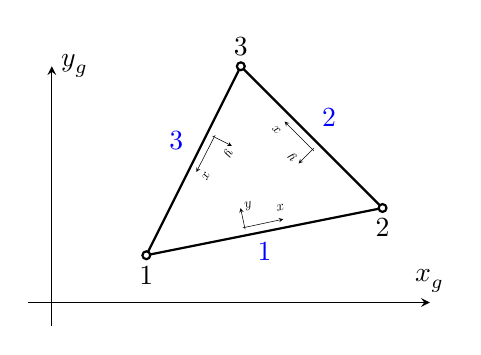
\begin{tikzpicture}[scale=6,>=stealth]
 \tikzstyle{elemnode} = [draw,circle,inner sep=1,fill=white]
 \newcommand{\lcoordsys}[1]{\draw[->] (-0.05,0) -- (1,0) node[above] {$x_{#1}$}; \draw[->] (0,-0.05) -- (0,0.5) node[right] {$y_{#1}$};}
 \draw[->] (-0.05,0) -- (0.8,0) node[above] {$x_g$};
 \draw[->] (0,-0.05) -- (0,0.5) node[right] {$y_g$};
 
 \draw[thick] 
     (0.2,0.1) node[elemnode] {} node[below] {1}
  -- (0.7,0.2) node[elemnode] {} node[below] {2} node[blue,midway,below] {1} coordinate[midway] (e1)
  -- (0.4,0.5) node[elemnode] {} node[above] {3} node[blue,midway,above right] {2} coordinate[midway] (e2)
  -- (0.2,0.1) node[blue,midway,above left] {3} coordinate[midway] (e3);

 \node[yshift=8] at (e1) {\rotatebox{12}{\scalebox{0.5}{\tikz{\lcoordsys{}}}}};
 \node[xshift=-9,yshift=-2] at (e2) {\rotatebox{135}{\scalebox{0.5}{\tikz{\lcoordsys{}}}}};
 \node[xshift=8,yshift=-1] at (e3) {\rotatebox{243}{\scalebox{0.5}{\tikz{\lcoordsys{}}}}};
\end{tikzpicture}

 \end{makeimage}
 \caption{Tr1CBS element. Node numbering, Side numbering and
 definition of local edge c.s.(a).}
 \label{Tr1CBSfig}
\end{figure}

\begin{elementsummary}{Tr1CBS}{linear triangular finite element for transient
incompressible flow analysis using cbs algorithm}{\optField{bsides}{ia} \optField{bcodes}{ia}}{Tr1CBS element summary}{Tr1CBSsummary}
\elementParam{Since the problem formulation requires to evaluate some boundary terms,
the element boundary edges should be specified as well as the types of
boundary conditions applied at these boundary edges. The boundary
edges (their numbers) are specified using \param{bsides} array. The
type of boundary condition(s) applied to corresponding boundary side
is determined by \param{bcodes} array. The available/supported
boundary codes are following: 1 for prescribed traction, 2 for
prescribed normal velocity, 4 for prescribed tangential velocity, and
8 for prescribed pressure. If the element side is subjected to a
combination of these fundamental types boundary conditions, the
corresponding code is obtained by summing up the corresponding codes.}
\elementDescription{Unknowns}{Two velocity components (V\_u and V\_v) and pressure (P\_f) are required in each node.}
\elementDescription{Approximation}{Equal order
approximation of velocity and pressure fields.}
\elementDescription{Integration}{exact}
\elementDescription{Features}{Constant boundary tractions are supported\footnote{In CBS algorithm formulation the prescribed traction
boundary condition leads indirectly to pressure boundary condition in
nodes associated to loaded edge. Such boundary condition is
represented by PrescribedTractionPressureBC. See section on boundary
conditions in OOFEM input manual.}. Body loads
representing the self-weight load are supported.}
\elementDescription{Status}{Untested}
\end{elementsummary}


%-----------------------------------------------------------------------------------------------
\clearpage
\subsection{2D SUPG/PSGP Elements}
\subsubsection{Tr1SUPG element}
\label{Tr1SUPG}
Represents the linear triangular finite element for transient
incompressible flow analysis using SUPG/PSPG stabilization with equal order
approximation of velocity and pressure fields. Each node has 3 degrees
of freedoms (two components of velocity and pressure).
The node numbering is anti-clockwise. The element features are summarized in Table~\ref{Tr1SUPGsummary}.

\begin{figure}[htb]
 \centering
 \begin{makeimage}
  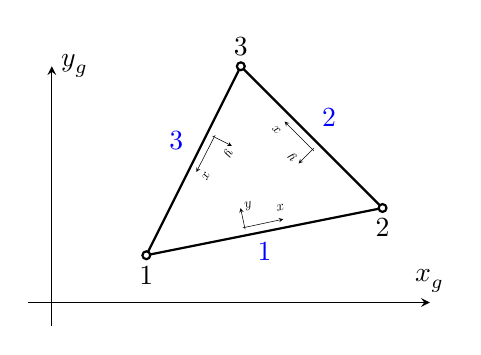
\begin{tikzpicture}[scale=6,>=stealth]
 \tikzstyle{elemnode} = [draw,circle,inner sep=1,fill=white]
 \newcommand{\lcoordsys}[1]{\draw[->] (-0.05,0) -- (1,0) node[above] {$x_{#1}$}; \draw[->] (0,-0.05) -- (0,0.5) node[right] {$y_{#1}$};}
 \draw[->] (-0.05,0) -- (0.8,0) node[above] {$x_g$};
 \draw[->] (0,-0.05) -- (0,0.5) node[right] {$y_g$};
 
 \draw[thick] 
     (0.2,0.1) node[elemnode] {} node[below] {1}
  -- (0.7,0.2) node[elemnode] {} node[below] {2} node[blue,midway,below] {1} coordinate[midway] (e1)
  -- (0.4,0.5) node[elemnode] {} node[above] {3} node[blue,midway,above right] {2} coordinate[midway] (e2)
  -- (0.2,0.1) node[blue,midway,above left] {3} coordinate[midway] (e3);

 \node[yshift=8] at (e1) {\rotatebox{12}{\scalebox{0.5}{\tikz{\lcoordsys{}}}}};
 \node[xshift=-9,yshift=-2] at (e2) {\rotatebox{135}{\scalebox{0.5}{\tikz{\lcoordsys{}}}}};
 \node[xshift=8,yshift=-1] at (e3) {\rotatebox{243}{\scalebox{0.5}{\tikz{\lcoordsys{}}}}};
\end{tikzpicture}

 \end{makeimage}
 \caption{Tr1SUPG element. Node numbering, Side numbering and
 definition of local edge c.s.(a).}
 \label{Tr1SUPG2fig}
\end{figure}

\begin{elementsummary}{Tr1SUPG}{linear triangular finite element for transient
incompressible flow analysis using SUPG/PSPG algorithm}{\optField{vof}{rn} \optField{pvof}{rn}}{Tr1SUPG element summary}{Tr1SUPGsummary}
\elementDescription{Unknowns}{Two velocity components (V\_u and V\_v) and pressure (P\_f) are required in each node.}
\elementDescription{Approximation}{Linear approximation of velocity and pressure fields.}
\elementDescription{Integration}{exact}
\elementDescription{Loads}{Constant boundary tractions are supported. Body loads
representing the self-weight load are supported.}
\elementDescription{Multi-fluid analysis}{The element has support for solving
problems with two immiscible fluids in
a fixed spatial domain. In the present implementation, a VOF and LevelSet tracking algorithms
are used to track the position of interface. In case of VOF tracking, an initial VOF fraction
(volume fraction of reference fluid) can be specified using
\param{vof} (default is zero). Element can also be marked as allways
filled with reference fluid (some form of source) using parameter
\param{pvof} which specifies the permanent VOF value. In case of LevelSet tracking, the initial levelset is specified using 
reference polygon (see corresponding levelset record in oofem input manual).
The material model should be of type \elemkeyword{twofluidmat}, that
supports modelling of two immiscible fluids.}
\elementDescription{Status}{Reliable}
\end{elementsummary}


\subsubsection{Tr21SUPG element}
\label{Tr21SUPG}
Implementation of P2P1 Taylor Hood element for transient incompressible flow analysis 
using SUPG and LSIC stabilization. It consists of globally continuous, piecewise quadratic functions for 
approximation in velocity space and globally continuous, piecewise linear functions for
approximation in pressure space. LBB condition is satisfied. There are 3 degrees
of freedom in vertices (two components of velocity and pressure), and 2 degrees of freedom
in edge nodes (two components of velocity only).
The node numbering is anti-clockwise, vertices are numbered first. The element features are summarized in Table~\ref{Tr21SUPGsummary}.

\begin{figure}[htb]
 \centering
 \begin{makeimage}
  \tikzstyle{elemnode} = [draw,circle,inner sep=1,fill=white]
\begin{tikzpicture}[scale=6,>=stealth]
 \draw[->] (-0.05,0) -- (0.8,0) node[above] {$x$};
 \draw[->] (0,-0.05) -- (0,0.5) node[right] {$y$};
 
 \draw[thick,xshift=-2] 
     (0.2,0.1) node[elemnode] {} node[below] {1}
  to[out=-10,in=210] node[elemnode,midway] {} node[below,midway] {4} (0.7,0.2) node[elemnode] {} node[below right] {2}
  to[out=110,in=-20] node[elemnode,midway] {} node[above right,midway] {5} (0.4,0.5) node[elemnode] {} node[above] {3}
  to[out=-90,in=40] node[elemnode,midway] {} node[above left,midway] {6} (0.2,0.1);
\end{tikzpicture}

 \end{makeimage}
 \caption{Tr21SUPG element - node and side numbering.}
 \label{Tr21SUPGfig}
\end{figure}

\begin{elementsummary}{Tr21SUPG}{P2P1 Taylor Hood element}{-}{Tr21SUPG element summary}{Tr21SUPGsummary}
\elementDescription{Unknowns}{Two velocity components (V\_u and V\_v) and pressure (P\_f) in vertices and two velocity components (V\_u and V\_v) in edge nodes are required.}
\elementDescription{Approximation}{Quadratic approximation of velocity and linear approximation of pressure fields.}
\elementDescription{Integration}{Integration is exact, each submatrix of element stiffness matrix is evaluated in proper number of
Gauss points. Submatrices connected with velocity are evaluated in 7 or 13 points, mixed velocity-pressure
submatrices in 3 or 7 points, submatrices connected with pressure in 3 points.}
\elementDescription{Loads}{Constant boundary tractions are supported. Body loads
representing the self-weight load are supported.}
\elementDescription{Multi-fluid analysis}{The element has no support for solving
problems with two immiscible fluids in a fixed spatial domain.}
\elementDescription{Status}{Reliable}
\end{elementsummary}


\subsubsection{Tr1SUPGAxi element}
\label{Tr1SUPGAxi}
Represents the linear triangular finite element for transient
incompressible flow analysis using SUPG/PSPG stabilization with equal order
approximation of velocity and pressure fields in 2d-axisymmetric setting. Each node has 3 degrees
of freedoms (two components of velocity and pressure). The y-axis is
axis of ratational symmetry. The node numbering is anti-clockwise. The element features are summarized in Table~\ref{Tr1SUPGAxisummary}.

\begin{figure}[htb]
 \centering
 \begin{makeimage}
  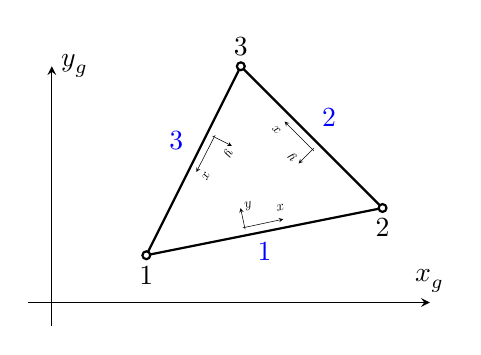
\begin{tikzpicture}[scale=6,>=stealth]
 \tikzstyle{elemnode} = [draw,circle,inner sep=1,fill=white]
 \newcommand{\lcoordsys}[1]{\draw[->] (-0.05,0) -- (1,0) node[above] {$x_{#1}$}; \draw[->] (0,-0.05) -- (0,0.5) node[right] {$y_{#1}$};}
 \draw[->] (-0.05,0) -- (0.8,0) node[above] {$x_g$};
 \draw[->] (0,-0.05) -- (0,0.5) node[right] {$y_g$};
 
 \draw[thick] 
     (0.2,0.1) node[elemnode] {} node[below] {1}
  -- (0.7,0.2) node[elemnode] {} node[below] {2} node[blue,midway,below] {1} coordinate[midway] (e1)
  -- (0.4,0.5) node[elemnode] {} node[above] {3} node[blue,midway,above right] {2} coordinate[midway] (e2)
  -- (0.2,0.1) node[blue,midway,above left] {3} coordinate[midway] (e3);

 \node[yshift=8] at (e1) {\rotatebox{12}{\scalebox{0.5}{\tikz{\lcoordsys{}}}}};
 \node[xshift=-9,yshift=-2] at (e2) {\rotatebox{135}{\scalebox{0.5}{\tikz{\lcoordsys{}}}}};
 \node[xshift=8,yshift=-1] at (e3) {\rotatebox{243}{\scalebox{0.5}{\tikz{\lcoordsys{}}}}};
\end{tikzpicture}

 \end{makeimage}
 \caption{Tr1SUPGAxi element. Node numbering, Side numbering and
 definition of local edge c.s.(a).}
 \label{Tr1SUPGAxifig}
\end{figure}

\begin{elementsummary}{Tr1SUPGAxi}{linear equal order approximation axisymmetric element}
  {\optField{vof}{rn}\optField{pvof}{rn}}{Tr1SUPGAxi element summary}{Tr1SUPGAxisummary}
\elementDescription{Unknowns}{Two velocity components (V\_u and V\_v) and pressure (P\_f) are required in each node.}
\elementDescription{Approximation}{Linear approximation of velocity and pressure fields.}
\elementDescription{Integration}{Gauss integration in seven point employed.}
\elementDescription{Loads}{Constant boundary tractions are supported. Body loads
representing the self-weight load are supported.}
\elementDescription{Multi-fluid analysis}{The element has support for solving
problems with two immiscible fluids in
a fixed spatial domain. In the present implementation, a VOF tracking algorithm
is used to track the position of interface. An initial VOF fraction
(volume fraction of reference fluid) can be specified using
\param{vof} (default is zero). Element can also be marked as always
filled with reference fluid (some form of source) using parameter
\param{pvof} which specifies the permanent VOF value. In this case,
the material model should be of type \elemkeyword{twofluidmat}, that
supports modelling of two immiscible fluids.}
\elementDescription{Status}{}
\end{elementsummary}


%-----------------------------------------------------------------------------------------------
\clearpage
\subsection{3D SUPG/PSGP Elements}
\subsubsection{Tet1\_3D\_SUPG element}
\label{PY1_3D_SUPG}
Represents 3D linear pyramid element for transient
incompressible flow analysis using SUPG/PSPG stabilization with equal order
approximation of velocity and pressure fields. Each node has 3 degrees
of freedoms (two components of velocity and pressure). The element features are summarized in Table~\ref{TET1SUPGsummary}.

\begin{figure}[htb]
 \centering
 \begin{makeimage}
  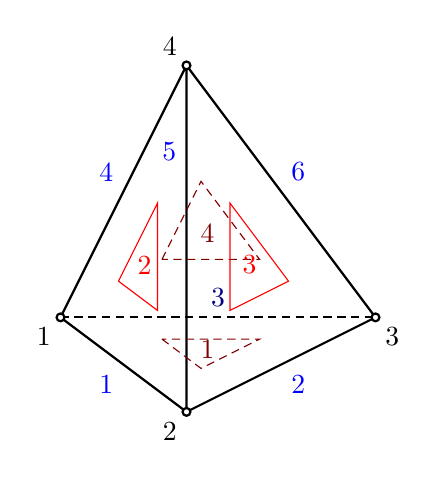
\begin{tikzpicture}[scale=4,>=stealth,x={(1cm,0cm)}, y={ (0.4cm,-0.3cm) }, z={(0.4cm,0.8cm)}]
 \tikzstyle{elemnode} = [draw=black,thick,fill=white,circle,inner sep=1]
 \tikzstyle{background} = [densely dashed]
 \newcommand{\fs}{0.23}
 
% Can't use rectangle in 3d
 \draw[thick,background] (0,0,0) -- (1,0,0) node[midway,above,blue!50!black] {3};
 \draw[thick] (0,0,1) -- (0,0,0) node[midway,above left,blue] {4}
                      -- (0,1,0) node[midway,below left,blue] {1} 
                      -- (1,0,0) node[midway,below right,blue] {2}
                      -- (0,0,1) node[midway,above right,blue] {6}
                      -- (0,1,0) node[near start,left,blue] {5};

% Nodes
 \node[elemnode] (n1) at (0,0,0) {}; \node[below left] at (n1) {1};
 \node[elemnode] (n2) at (0,1,0) {}; \node[below left] at (n2) {2};
 \node[elemnode] (n3) at (1,0,0) {}; \node[below right] at (n3) {3};
 \node[elemnode] (n4) at (0,0,1) {}; \node[above left] at (n4) {4};

% Faces
 \draw[red!50!black,background] (\fs,\fs,0) -- (\fs,1-2*\fs,0) -- (1-2*\fs,\fs,0) -- cycle;
 \node[red!50!black] at (1/3,1/3,0) {1};
 \draw[red!50!black,background] (\fs,0,\fs) -- (\fs,0,1-2*\fs) -- (1-2*\fs,0,\fs) -- cycle;
 \node[red!50!black] at (1/3,0,1/3) {4};

 \draw[red] (0,\fs,\fs) -- (0,\fs,1-2*\fs) -- (0,1-2*\fs,\fs) -- cycle;
 \node[red] at (0,1/3,1/3) {2};
 \draw[red] (1-2*\fs,\fs,\fs) -- (\fs,1-2*\fs,\fs) -- (\fs,\fs,1-2*\fs) -- cycle;
 \node[red] at (1/3,1/3,1/3) {3};


\end{tikzpicture}

 \end{makeimage}
 \caption{Tet1\_3D\_SUPG element.}
 \label{PY1_3D_SUPGfig}
\end{figure}

\begin{elementsummary}{TET1SUPG}{linear equal order approximation axisymmetric element}
  {\optField{vof}{rn}\optField{pvof}{rn}}{TET1SUPG element summary}{TET1SUPGsummary}
\elementDescription{Unknowns}{Three velocity components (V\_u, V\_v, and V\_w) and pressure (P\_f) are required in each node.}
\elementDescription{Approximation}{Linear approximation of velocity and pressure fields.}
\elementDescription{Integration}{exact}
\elementDescription{Loads}{Constant boundary tractions are supported. Body loads
representing the self-weight load are supported.}
\elementDescription{Multi-fluid analysis}{The element has support for solving
problems with two immiscible fluids in
a fixed spatial domain. In the present implementation, a LevelSet tracking algorithm
is used to track the position of interface. 
The material model should be of type \elemkeyword{twofluidmat}, that
supports modelling of two immiscible fluids.}
\elementDescription{Status}{}
\end{elementsummary}


% References;
\printbibliography

\end{document}


